% !TeX program = xelatex
% !TeX encoding = utf8
\documentclass[12pt,a4paper]{article}
\usepackage{fontspec}
\usepackage{polyglossia}
\setdefaultlanguage{vietnamese}
% Use the system-installed Times New Roman for report text on both operating systems.
\setmainfont{Times New Roman}
\setsansfont{Times New Roman}
\setmonofont{NotoSansMono}[
    Path=../../assets/fonts/,
    Extension=.ttf,
    UprightFont=*-Regular,
    BoldFont=*-Bold
]
\usepackage{amsmath,amssymb,amsfonts,amsthm}
\usepackage{geometry}
\usepackage{graphicx}
% Image paths are relative to tex-report/code/; compile from this directory.
\usepackage{booktabs}
\usepackage{array}
\usepackage{multirow}
\usepackage{adjustbox}
\usepackage{float}
\usepackage{listings}
\usepackage{url}
\usepackage{xcolor}
\usepackage{colortbl}
\usepackage{tabularx}
\usepackage{ragged2e}
\usepackage{tikz}
\usetikzlibrary{shapes.geometric, arrows, positioning}
\usepackage{setspace}
\geometry{a4paper, left=2.5cm, right=2cm, top=2.5cm, bottom=2.5cm}
\setstretch{1}
\setlength{\parskip}{0pt}
\setlength{\parindent}{1.5em}
\usepackage{fancyhdr}
\pagestyle{fancy}
\fancyhf{}
\fancyhead[L]{\small BÁO CÁO CUỐI KỲ -- THỐNG KÊ TÍNH TOÁN}
\fancyhead[R]{\small Khoảng tin cậy Bootstrap}
\renewcommand{\headrulewidth}{0.4pt}
\setlength{\headheight}{14pt}

\fancypagestyle{plain}{%
	\fancyhf{}%
	\fancyhead[L]{\small BÁO CÁO CUỐI KỲ -- THỐNG KÊ TÍNH TOÁN}%
	\fancyhead[R]{\small Khoảng tin cậy Bootstrap}%
	\renewcommand{\headrulewidth}{0.4pt}%
}

\usepackage{enumitem}
\setlist[itemize]{
	leftmargin=1.7em,
	itemsep=0.3em,
	topsep=0.3em,
	parsep=0pt,
	partopsep=0pt
}
\setlist[enumerate]{
	leftmargin=2em,
	itemsep=0.3em,
	topsep=0.3em,
	parsep=0pt,
	partopsep=0pt
}

\usepackage{titlesec}
\titlelabel{\thetitle.\hspace{0.2em}}
\titlespacing*{\section}{0pt}{1.2ex plus .3ex minus .2ex}{0.6ex}
\titlespacing*{\subsection}{0pt}{1ex plus .2ex minus .2ex}{0.4ex}
\titlespacing*{\subsubsection}{0pt}{0.8ex plus .2ex minus .2ex}{0.3ex}

\usepackage[ruled,vlined,linesnumbered]{algorithm2e}
\counterwithin{algocf}{section}
\SetKwInput{Input}{Đầu vào}
\SetKwInput{Output}{Đầu ra}

% Định nghĩa môi trường toán học
\theoremstyle{definition}
\newtheorem{theorem}{Định lý}[section]
\newtheorem{definition}[theorem]{Định nghĩa}
\newtheorem{property}[theorem]{Tính chất}
\newtheorem{lemma}[theorem]{Bổ đề}
\newtheorem{remark}[theorem]{Nhận xét}
\newtheorem{example}[theorem]{Ví dụ}
\numberwithin{equation}{section}
\counterwithin{table}{section}
\counterwithin{figure}{section}

% Cấu hình hiển thị code R
\definecolor{codegreen}{rgb}{0.00,0.60,0.05}
\definecolor{codegray}{rgb}{0.5,0.5,0.5}
\definecolor{codepurple}{rgb}{0.00,0.20,0.67}
\definecolor{backcolour}{rgb}{0.95,0.95,0.92}

\lstdefinestyle{Rstyle}{
	backgroundcolor=\color{backcolour},
	commentstyle=\color{codegreen},
	keywordstyle=\color{magenta},
	numberstyle=\tiny\color{codegray},
	stringstyle=\color{codepurple},
	basicstyle=\ttfamily\footnotesize,
	breakatwhitespace=false,
	breaklines=true,
	captionpos=b,
	keepspaces=true,
	numbers=none,
	showspaces=false,
	showstringspaces=false,
	showtabs=false,
	tabsize=2,
	language=R
}
\lstset{style=Rstyle}



\begin{document}

\justifying

	% ==================== TRANG BÌA ====================
	\begin{titlepage}
		\begin{tikzpicture}[remember picture, overlay]
			\draw[line width=1.5pt]
				([xshift=20mm, yshift=-20mm]current page.north west)
				rectangle
				([xshift=-15mm, yshift=20mm]current page.south east);
			\draw[line width=0.6pt]
				([xshift=21.5mm, yshift=-21.5mm]current page.north west)
				rectangle
				([xshift=-16.5mm, yshift=21.5mm]current page.south east);
		\end{tikzpicture}
		\centering
		{\small TỔNG LIÊN ĐOÀN LAO ĐỘNG VIỆT NAM\par}
		\vspace{0.5cm}
		{\large\bfseries TRƯỜNG ĐẠI HỌC TÔN ĐỨC THẮNG\par}
		\vspace{0.1cm}
		{\large\bfseries KHOA TOÁN – THỐNG KÊ\par}
		\vspace{0.35cm}
		
\includegraphics[width=7cm]{../../assets/tdtu-logo.jpg}\par
		\vspace{0.8cm}

		{\Large \bfseries BÁO CÁO CUỐI KỲ\par}
		\vspace{0.2cm}
		{\small MÔN HỌC: THỐNG KÊ TÍNH TOÁN – MÃ MH: C03107\par}
		{\small HỌC KỲ: 1/2026-2027\par}
		\vspace{0.8cm}

		{\Large \bfseries KHOẢNG TIN CẬY BOOTSTRAP CHUẨN TẮC VÀ BOOTSTRAP CƠ BẢN:\par}
		\vspace{0.3cm}
		{\large \bfseries CƠ SỞ LÝ THUYẾT, PHƯƠNG PHÁP XÂY DỰNG VÀ ĐÁNH GIÁ\par}
		\vspace{1.8cm}

		\begin{center}
			\textbf{Giảng viên hướng dẫn:} ThS. Bùi Thùy Trang \\[0.2cm]
			\textbf{Nhóm thực hiện:} Nhóm D \\[0.1cm]
			\begin{tabular}{r l}
				MSSV & | Họ và Tên \\
				C2400121 & | Phan Trí Thịnh \\
				C2400115 & | Ngô Cẩm Quí \\
				C2400203 & | Nguyễn Văn Kiệt \\
				C2400199 & | Trần Quốc Khang \\
			\end{tabular}
		\end{center}

		\vfill
		{\small TP. HỒ CHÍ MINH, NGÀY 29 THÁNG 9 NĂM 2026\par}
	\end{titlepage}

	\newpage
	\pagenumbering{roman}
	\setcounter{page}{1}

	% ==================== BẢNG PHÂN CÔNG ====================
	\section*{BẢNG PHÂN CÔNG NHIỆM VỤ}
	\vspace{0.3cm}

	\begin{center}
		\small
		\renewcommand{\arraystretch}{1.25}
		\setlength{\tabcolsep}{5pt}
		\begin{tabular}{|c|c|p{3.0cm}|p{6.8cm}|c|}
			\hline
			\textbf{STT} & \textbf{MSSV} & \textbf{Họ và tên} & \textbf{Nhiệm vụ} & \textbf{Hoàn thành} \\
			\hline
			1 & C2400121 & Phan Trí Thịnh &
			\textbf{Phần 1:} Giới thiệu tổng quan và bối cảnh nghiên cứu.\par\smallskip
			\textbf{Phần 2:} Cơ sở toán học ECDF, nguyên lý Plug-in và thuật toán Monte Carlo. &
			100\% \\
			\hline
			2 & C2400115 & Ngô Cẩm Quí &
			\textbf{Phần 3:} Normal CI, Basic CI và Quantile Flipping.\par\smallskip
			\textbf{Phần 4:} So sánh Normal CI và Basic CI. &
			100\% \\
			\hline
			3 & C2400203 & Nguyễn Văn Kiệt &
			\textbf{Phần 5:} Xây dựng và phân tích hai ví dụ Bootstrap (mẫu đối xứng, mẫu lệch phải); liệt kê chính xác bằng R.\par\smallskip
			\textbf{Phần 6:} Mô phỏng Monte Carlo bằng R. &
			100\% \\
			\hline
			4 & C2400199 & Trần Quốc Khang &
			\textbf{Phần 7:} Phân tích ứng dụng trong bài báo.\par\smallskip
			\textbf{Phần 8:} Percentile CI và tính bất biến.\par\smallskip
			\textbf{Phần 9:} Kết luận. &
			100\% \\
			\hline
		\end{tabular}
	\end{center}

	\vspace{1cm}

	\begin{flushright}
		\textit{TP. Hồ Chí Minh, ngày 29 tháng 09 năm 2026}\\[0.2cm]
		\textbf{Nhóm trưởng Nhóm D}\\[1.2cm]
	\end{flushright}

	\newpage

	% ==================== LỜI CẢM ƠN ====================
	\addcontentsline{toc}{section}{LỜI CẢM ƠN}

	\begin{center}
		{\Large\bfseries LỜI CẢM ƠN}
	\end{center}

	\vspace{0.5cm}
	Nhóm D xin chân thành cảm ơn ThS. Bùi Thùy Trang, giảng viên môn Thống kê Tính toán (C03107), Khoa Toán – Thống kê, Trường Đại học Tôn Đức Thắng, vì những hướng dẫn trong quá trình học tập và thực hiện báo cáo. Tài liệu bài giảng về Bootstrap và Jackknife là nguồn tham khảo chính cho phần cơ sở lý thuyết của nhóm~\cite{buithuytrang2026,rizzo2019}.

Qua quá trình tìm hiểu các khoảng tin cậy Bootstrap và triển khai mô phỏng bằng R, nhóm có cơ hội vận dụng kiến thức của học phần vào các ví dụ và kịch bản cụ thể. Báo cáo vẫn còn những hạn chế; nhóm mong nhận được góp ý của cô để tiếp tục hoàn thiện. Nhóm xin chân thành cảm ơn cô!

	\newpage

	% ==================== LỜI MỞ ĐẦU ====================
	\addcontentsline{toc}{section}{LỜI MỞ ĐẦU}

	\begin{center}
		{\Large\bfseries LỜI MỞ ĐẦU}
	\end{center}

	\vspace{0.5cm}
	Trong suy diễn thống kê, khoảng tin cậy thường được xây dựng dựa trên giả định về phân phối hoặc các xấp xỉ tiệm cận, chẳng hạn xấp xỉ Chuẩn khi cỡ mẫu đủ lớn. Với mẫu nhỏ, phân phối lệch hoặc dữ liệu có ngoại lai, các xấp xỉ này có thể chưa phù hợp và xác suất bao phủ thực tế có thể khác mức danh nghĩa~\cite{buithuytrang2026,rizzo2019,efron1993,davison1997}.

Bootstrap thay phân phối tổng thể chưa biết bằng phân phối thực nghiệm của mẫu và lấy mẫu lại có hoàn lại. Phân phối Bootstrap có điều kiện này được dùng để xấp xỉ phân phối lấy mẫu của thống kê; khi chỉ tạo hữu hạn bản sao, ta còn có xấp xỉ Monte Carlo của phân phối Bootstrap~\cite{efron1979,efron1993}. Chất lượng xấp xỉ phụ thuộc vào dữ liệu, thống kê và cách lấy mẫu lại.

	Báo cáo gồm chín phần, trình bày cơ sở lý thuyết, ví dụ, mô phỏng và ứng dụng:
	\begin{itemize}
		\item \textbf{Phần 1: Giới thiệu tổng quan và bối cảnh nghiên cứu:} Nêu động lực, mục tiêu, phạm vi và một số mốc phát triển của kỹ thuật lấy mẫu lại (resampling)~\cite{efron1979}.
		\item \textbf{Phần 2: Cơ sở toán học của ECDF và thuật toán Monte Carlo:} Trình bày các tính chất của $F_n$, nguyên lý Plug-in và mô hình xác suất Bootstrap~\cite{buithuytrang2026,rizzo2019}.
		\item \textbf{Phần 3: Phương pháp xây dựng khoảng tin cậy Normal CI và Basic CI:} Trình bày cơ sở, công thức và thuật toán xây dựng hai khoảng; với Basic CI, giải thích phép đảo phân vị (quantile flipping)~\cite{rizzo2019,efron1993}.
		\item \textbf{Phần 4: So sánh Normal CI và Basic CI:} So sánh giả định và cách hai phương pháp phản ánh độ lệch của phân phối~\cite{davison1997}.
		\item \textbf{Phần 5: Ví dụ Bootstrap:} Phân tích mẫu đối xứng và mẫu lệch phải bằng cách liệt kê các mẫu Bootstrap trong R.
		\item \textbf{Phần 6: Mô phỏng Monte Carlo bằng R:} Đánh giá coverage và độ dài trung bình trong bốn kịch bản đã xác định.
		\item \textbf{Phần 7: Ứng dụng trong bài báo khoa học:} Trình bày cách Deng và cộng sự dùng khoảng BCa để phân tích relative validity~\cite{deng2013}.
		\item \textbf{Phần 8: Percentile CI và tính bất biến:} So sánh ba phương pháp và xét tính bất biến dưới phép biến đổi tham số $g(\theta)$~\cite{efron1993}.
		\item \textbf{Phần 9: Kết luận và khuyến nghị:} Tóm tắt kết quả và nêu khuyến nghị trong phạm vi các ví dụ, kịch bản đã xét.
	\end{itemize}

	\newpage

	% ==================== MỤC LỤC TỰ ĐỘNG ====================
	\renewcommand{\contentsname}{\Large\bfseries MỤC LỤC}
	\tableofcontents

	\newpage
	\pagenumbering{arabic}
	\setcounter{page}{1}

	% ==================== PHẦN 1 ====================

	\section{GIỚI THIỆU TỔNG QUAN VÀ BỐI CẢNH NGHIÊN CỨU}

	\subsection{Bối cảnh và động lực nghiên cứu}
	Trong lý thuyết suy diễn thống kê truyền thống, việc xây dựng khoảng tin cậy cho một tham số tổng thể $\theta$ (như trung bình $\mu$, phương sai $\sigma^2$, hay tỷ số Odds Ratio) thường dựa vào các giả định phân phối tham số chặt chẽ (chẳng hạn như giả định mẫu rút ra từ phân phối Chuẩn $N(\mu, \sigma^2)$) hoặc dựa trên các kết quả tiệm cận khi kích thước mẫu $n \to \infty$ thông qua Định lý Giới hạn Trung tâm (CLT)~\cite{buithuytrang2026,rizzo2019,quyen2025}.

	Trong một số ứng dụng, dữ liệu có thể không đáp ứng tốt các giả định này; một số tình huống thường gặp gồm~\cite[tr. 11--14, 258--261]{efron1993}:
	\begin{itemize}
		\item \textbf{Cỡ mẫu nhỏ:} Chi phí, độ hiếm của đối tượng hoặc thời gian thu thập có thể giới hạn cỡ mẫu. Khi đó, xấp xỉ tiệm cận có thể chưa chính xác; mức độ ảnh hưởng phụ thuộc vào bài toán cụ thể~\cite[tr. 258--261]{efron1993}.
		\item \textbf{Phân phối lệch hoặc có ngoại lai:} Thu nhập, chi phí bồi thường bảo hiểm, thời gian sống sót và nồng độ độc tố có thể có phân phối lệch hoặc đuôi dày~\cite[tr. 11--15]{davison1997}.
		\item \textbf{Thống kê ước lượng phức tạp:} Trong nhiều bài toán thực tế, nhà nghiên cứu quan tâm đến các tham số không có công thức phương sai giải tích đơn giản, chẳng hạn như Trung vị (Median), Hệ số Gini, Tỷ số rủi ro (Hazard Ratio), hay các trọng số tối ưu trong danh mục đầu tư~\cite[tr. 14--16, 38--41]{efron1993}.
	\end{itemize}

	Khi các giả định của phương pháp cổ điển không phù hợp, khoảng thu được có thể phản ánh chưa đúng độ bất định và coverage thực tế có thể khác mức danh nghĩa $1-\alpha$. Bootstrap là một phương pháp khác để ước lượng độ bất định, nhưng hiệu năng của khoảng vẫn phụ thuộc vào dữ liệu và cách lấy mẫu lại~\cite{efron1979,davison1997}.

	\subsection{Mục tiêu và phạm vi nghiên cứu}
	Báo cáo tập trung vào hai phương pháp khoảng tin cậy Bootstrap: \textbf{Normal CI} và \textbf{Basic CI}~\cite{buithuytrang2026,rizzo2019}. Percentile CI được đưa vào phần mở rộng.

	Báo cáo hướng đến các mục tiêu sau:
	\begin{enumerate}
		\item \textbf{Trình bày cơ sở toán học:} Giới thiệu ECDF, một số tính chất cơ bản, nguyên lý Plug-in và mô hình xác suất Bootstrap~\cite{rizzo2019,efron1993}.
		\item \textbf{So sánh phương pháp:} Trình bày công thức Normal CI và Basic CI, đồng thời giải thích phép biến đổi phân vị trong Basic CI~\cite{rizzo2019,davison1997,justus2024}.
		\item \textbf{Minh họa và mô phỏng:} Phân tích hai ví dụ bằng cách liệt kê chính xác trong R; mô phỏng Monte Carlo với $K=10{,}000$ lần lặp để ước lượng coverage và độ dài trung bình trong bốn kịch bản.
		\item \textbf{Ứng dụng và mở rộng:} Mô tả một ứng dụng BCa trong bài báo khoa học, so sánh Percentile CI và khảo sát tính bất biến dưới phép biến đổi $g(\theta)$; khuyến nghị giới hạn theo kết quả đã trình bày~\cite{efron1993,deng2013}.
	\end{enumerate}

	Phạm vi lý thuyết tập trung vào dữ liệu i.i.d. và ba phương pháp Normal, Basic, Percentile CI. Phần mô phỏng chỉ xét hai phân phối, hai cỡ mẫu và các thiết lập nêu tại Phần 6; kết quả không đại diện cho mọi dạng dữ liệu~\cite[tr. 18--22]{davison1997}.

	\subsection{Bối cảnh ra đời của thống kê phi tham số và resampling}
	Sự phát triển của một số phương pháp lấy mẫu lại gắn với tiến bộ về tính toán. Các mốc tiêu biểu gồm:
	\begin{itemize}
		\item \textbf{Kiểm định hoán vị (thập niên 1930):} Ronald Fisher (1935) và E. J. G. Pitman (1937) phát triển các phép kiểm định dựa trên việc xét các cách gán nhãn lại dữ liệu. Khi số cấu hình tăng theo giai thừa của cỡ mẫu, việc liệt kê đầy đủ bị giới hạn bởi chi phí tính toán~\cite{efron1979,efron1993}.
		\item \textbf{Jackknife (1949, 1958):} Maurice Quenouille (1949) đề xuất loại lần lượt từng quan sát để giảm độ chệch của ước lượng. John Tukey (1958) mở rộng phương pháp này để ước lượng phương sai và đặt tên là Jackknife. Phương pháp có hạn chế với một số thống kê không trơn, chẳng hạn trung vị~\cite{efron1979,efron1993}.
		\item \textbf{Bootstrap (1979):} Efron giới thiệu phương pháp trong bài báo \textit{"Bootstrap Methods: Another Look at the Jackknife"}. Bootstrap thay phân phối tổng thể bằng phân phối thực nghiệm của mẫu gốc rồi lấy mẫu lại có hoàn lại. Khi không liệt kê toàn bộ các mẫu, mô phỏng Monte Carlo được dùng để xấp xỉ phân phối Bootstrap~\cite{efron1979,efron1993}.
	\end{itemize}


	% ==================== PHẦN 2 ====================

	\newpage
	\section{CƠ SỞ TOÁN HỌC CỦA ECDF VÀ THUẬT TOÁN MONTE CARLO}

	\subsection{Phân phối thực nghiệm (\textit{Empirical Distribution}) và các đặc trưng đại số}
	Cho $X_{1:n}=(X_1,\ldots,X_n)$ là mẫu ngẫu nhiên gồm $n$ biến i.i.d.\ có
    hàm phân phối $F(t)=\mathbb P(X_1\le t)$. Ký hiệu $x=(x_1,\ldots,x_n)$
    là một mẫu đã quan sát từ $X_{1:n}$~\cite[Chương 4]{buithuytrang2026}.

    \begin{definition}[\textbf{Hàm phân phối thực nghiệm ECDF}]
        Với mỗi $t\in\mathbb R$, $F_n(t)$ là đại lượng ngẫu nhiên trước khi
        quan sát, còn $F_{n,x}(t)$ là giá trị tính từ mẫu đã quan sát~\cite[Chương 4]{buithuytrang2026}:
        \begin{equation}
            \begin{aligned}
                F_n(t)&=\frac1n\sum_{i=1}^n \mathbb I_{(-\infty,t]}(X_i),\\
                F_{n,x}(t)&=\frac1n\sum_{i=1}^n\mathbb I_{(-\infty,t]}(x_i)
                    =\frac{\#\{i:x_i\le t\}}{n}.
            \end{aligned}
        \end{equation}
        trong đó $\mathbb{I}_A(\cdot)$ là hàm chỉ thị (indicator function):
		\begin{equation}
			\mathbb{I}_A(y) = \begin{cases}
				1 & \text{nếu } y \in A \\
				0 & \text{nếu } y \notin A
			\end{cases}
		\end{equation}
	\end{definition}
		Xét mẫu minh họa $x=(12,15,18,21,24)$. Tại mỗi giá trị quan sát
		$x_{(i)}$, hàm ECDF bằng tỷ lệ số quan sát không vượt quá giá trị đó:

		\begin{table}[htbp]
			\centering
			\caption{Tính hàm phân phối thực nghiệm từ một mẫu}
			\label{tab:ecdf-values}
			\begin{tabular}{ccc}
				\toprule
				Giá trị $x_{(i)}$ & Số quan sát $\leq x_{(i)}$ & $F_{n,x}(x_{(i)})$ \\
				\midrule
				12 & 1 & 0.2 \\
				15 & 2 & 0.4 \\
				18 & 3 & 0.6 \\
				21 & 4 & 0.8 \\
				24 & 5 & 1.0 \\
				\bottomrule
			\end{tabular}
		\end{table}

	\textbf{Các tính chất xác suất của $F_n(t)$:}
	\begin{enumerate}
		\item \textbf{Tính chất phân phối nhị thức:}
		Với $t$ cố định, đặt $Y_i=\mathbf{1}\{X_i\le t\}$. Các $Y_i$ là
        biến Bernoulli độc lập cùng xác suất thành công $F(t)$, nên:
        \begin{equation}
			nF_n(t)=\sum_{i=1}^{n}Y_i
			\sim \operatorname{Binomial}\bigl(n,F(t)\bigr).
		\end{equation}
		\item \textbf{Tính không chệch (Unbiasedness):} Kỳ vọng của $F_n(t)$ đúng bằng phân phối tổng thể thực sự $F(t)$ tại mọi điểm $t$~\cite[Chương 4]{buithuytrang2026}:
		\begin{equation}
			\mathbb{E}[F_n(t)] = \mathbb{E}\left[\frac{1}{n}\sum_{i=1}^n Y_i\right] = \frac{1}{n} \cdot n F(t) = F(t)
		\end{equation}
		\item \textbf{Phương sai và hội tụ tại từng điểm:} Phương sai của $F_n(t)$ tiến về 0 khi $n \to \infty$~\cite[Chương 4]{buithuytrang2026}:
		\begin{equation}
			\text{Var}\left(F_n(t)\right) = \text{Var}\left(\frac{1}{n}\sum_{i=1}^n Y_i\right) = \frac{n F(t)(1 - F(t))}{n^2} = \frac{F(t)(1 - F(t))}{n} \xrightarrow{n \to \infty} 0
		\end{equation}
		Với mỗi $t$ cố định, bất đẳng thức Chebyshev cho thấy:
		\begin{equation}
			\mathbb{P}\left(\left|F_n(t)-F(t)\right|>\varepsilon\right)
			\leq
			\frac{F(t)(1-F(t))}{n\varepsilon^2}
			\longrightarrow 0.
		\end{equation}
		Vì vậy, với mỗi $t$ cố định, $F_n(t)$ hội tụ theo xác suất về $F(t)$.
		\item \textbf{Định lý Glivenko-Cantelli:} Hàm phân phối thực nghiệm $F_n(t)$ hội tụ đều về hàm phân phối tổng thể $F(t)$ hầu chắc chắn trên toàn bộ đường thẳng thực $\mathbb{R}$~\cite[tr. 10--12]{efron1993}:
		\begin{equation}
			\mathbb{P}\left( \lim_{n \to \infty} \sup_{t \in \mathbb{R}} |F_n(t) - F(t)| = 0 \right) = 1
		\end{equation}

	\newpage
		\item \textbf{Minh họa bằng mô phỏng R:} Mô phỏng dưới đây lấy mẫu từ phân phối Chuẩn $N(0,1)$ với các cỡ mẫu $n=10,30,100,1000$, sau đó so sánh ECDF với hàm phân phối lý thuyết $F(t)=\Phi(t)$.

	\begin{lstlisting}[style=Rstyle, caption={Mô phỏng ECDF}]
set.seed(2026)
n_sizes <- c(10, 30, 100, 1000)
cols <- c("red", "orange", "blue", "forestgreen")

curve(pnorm(x), from = -3, to = 3, lwd = 2, ylab = "F(t)", xlab = "t")
for (i in seq_along(n_sizes)) {
  lines(ecdf(rnorm(n_sizes[i])), col = cols[i], verticals = TRUE, do.points = FALSE)
}
legend("topleft", legend = c("True Normal", paste("n =", n_sizes)),
       col = c("black", cols), lwd = 2, bty = "n")
	\end{lstlisting}
	\end{enumerate}


	\subsection{Nguyên lý Plug-in và Mô hình Không gian Xác suất Bootstrap}

	\begin{definition}[\textbf{Nguyên lý Plug-in}]
		Nếu $\theta=T(F)$ là một phiếm hàm của phân phối tổng thể, ước lượng
        plug-in là $T(F_n)$. Sau khi quan sát $X_{1:n}=x$, giá trị ước lượng
        là $T(F_{n,x})$~\cite{buithuytrang2026,efron1993}.
        \begin{equation}
            \hat\theta_n=T(F_n),\qquad
            \hat\theta_n(x)=T(F_{n,x}).
        \end{equation}
    \end{definition}

    \textbf{Hai ví dụ plug-in trên mẫu đã quan sát:}
    \begin{itemize}
        \item Với trung bình, $F_{n,x}$ gán trọng số $1/n$ cho mỗi vị trí $i$.
        Nếu nhiều vị trí có cùng giá trị, các trọng số của chúng được cộng lại.
        Do đó~\cite[Chương 4]{buithuytrang2026}:
        \begin{equation}
            \mu(F_{n,x})=\int u\,dF_{n,x}(u)=\frac1n\sum_{i=1}^n x_i=\bar x.
        \end{equation}
        \item Với phương sai, thay $F$ bằng $F_{n,x}$ và trung bình tổng thể
        bằng $\bar x$ cho phương sai thực nghiệm với mẫu số $n$~\cite[Chương 4]{buithuytrang2026}:
        \begin{equation}
            \sigma^2(F_{n,x})=\int (u-\bar x)^2\,dF_{n,x}(u)
            =\frac1n\sum_{i=1}^n (x_i-\bar x)^2.
        \end{equation}
    \end{itemize}

    \newpage

    \textbf{Sơ đồ Tương đương trong "Thế giới Bootstrap":}
	Trong cơ chế Bootstrap, phân phối thực nghiệm $F_{n,x}$ đóng vai trò phân phối tổng thể thay thế; mẫu quan sát $x$ vì vậy được xem như một tổng thể giả lập~\cite[tr. 34--36]{efron1993}:
	\begin{equation}
		\begin{array}{r c l c l c l}
			\textbf{Thế giới thực:}
			& F
			& \xrightarrow{\text{lấy mẫu ngẫu nhiên}}
			& X_{1:n}
			& \xrightarrow{\text{tính thống kê}}
			& \hat{\theta}_n
			& \\[1.2em]

			\textbf{Thế giới Bootstrap:}
			& F_{n,x}
			& \xrightarrow{\text{lấy mẫu có hoàn lại}}
			& X_{1:n}^*
			& \xrightarrow{\text{tính thống kê}}
			& \hat{\theta}_n^*
			&
		\end{array}
	\end{equation}

	\subsection{Mẫu Bootstrap và Thuật toán Lấy mẫu lại Monte Carlo}

	Cho trước $X_{1:n}=x$, rút độc lập $n$ chỉ số $J_1,\ldots,J_n$,
    mỗi chỉ số đều trên $\{1,\ldots,n\}$, rồi đặt $X_i^*=x_{J_i}$.
    Ký hiệu $\mathbb P^*$ là xác suất có điều kiện theo mẫu gốc.
    Khi đánh giá tại mẫu $x$:
    \[
        \mathbb P^*(J_i=j)=\frac1n,\qquad
        \mathbb P^*(X_i^*=v)=\frac{\#\{j:x_j=v\}}{n}.
    \]
    Vì vậy, các $X_i^*$ có phân phối có điều kiện $F_{n,x}$.
    Chẳng hạn, với $x=(1,1,1,9)$, mỗi vị trí có xác suất $1/4$, còn giá trị
    $1$ có xác suất $3/4$. ECDF $F_n^*$ của mẫu lấy lại được tính từ các
    $X_i^*$. Dùng cùng quy tắc thống kê $t$ trên mẫu đó cho bản sao
    $\hat\theta_n^*=t(X_{1:n}^*)$. Với ước lượng plug-in, bản sao là $T(F_n^*)$~\cite{buithuytrang2026,rizzo2019,efron1993}.

    Nếu $n$ quan sát ban đầu đôi một khác nhau, số mẫu Bootstrap khác
	nhau khi xem mỗi mẫu như một đa tập, không xét thứ tự, là
	$\binom{2n-1}{n}$. Với $n=20$, con số này bằng
	$\binom{39}{20}=68{,}923{,}264{,}410$. Số lượng lớn này cho thấy việc
	liệt kê toàn bộ các cấu hình thường không thuận tiện, vì vậy ta dùng
	mô phỏng Monte Carlo để xấp xỉ phân phối Bootstrap~\cite{rizzo2019,efron1993}.

	\begin{algorithm}[H]
        \Input{Mẫu đã quan sát $x=(x_1,\dots,x_n)$, hàm thống kê $t(\cdot)$ và $B\ge 2$.}
        \Output{Giá trị $\hat\theta_n(x)$, dãy bản sao $(T_1^*,\ldots,T_B^*)$,
        ước lượng phương sai $\widehat V_B^*$ và sai số chuẩn $\widehat{se}^*$.}
        Tính $\hat\theta_n(x)=t(x)$\;
        \For{$b=1,\ldots,B$}{
            Rút độc lập $J_1^{(b)},\ldots,J_n^{(b)}$ đều trên $\{1,\ldots,n\}$\;
            Lập mẫu lấy lại $X^{*(b)}=(x_{J_1^{(b)}},\ldots,x_{J_n^{(b)}})$\;
            Tính và lưu $T_b^*=t(X^{*(b)})$\;
        }
        Tính $\bar T_B^*=\frac1B\sum_{b=1}^B T_b^*$\;
        Tính $\widehat V_B^*=\frac1{B-1}\sum_{b=1}^B(T_b^*-\bar T_B^*)^2$,
        rồi lấy $\widehat{se}^*=\sqrt{\widehat V_B^*}$\;
        \Return $\hat\theta_n(x),\ (T_b^*)_{b=1}^B,\ \widehat V_B^*,\ \widehat{se}^*$\;
        \caption{Lấy mẫu lại Monte Carlo và ước lượng sai số chuẩn Bootstrap}
        \label{alg:bootstrap-monte-carlo}
    \end{algorithm}

    Với mẫu gốc đã cố định, các lần lặp dùng dãy chỉ số độc lập nên
    $T_1^*,\ldots,T_B^*$ độc lập cùng phân phối.
    Đặt $\mu^*=\mathbb E^*[T_1^*]$ và $V^*=\operatorname{Var}^*(T_1^*)$
    khi moment bậc hai hữu hạn. Khi đó
    \[
        \sum_{b=1}^B(T_b^*-\bar T_B^*)^2
        =\sum_{b=1}^B(T_b^*-\mu^*)^2-B(\bar T_B^*-\mu^*)^2.
    \]
    Vì $\operatorname{Var}^*(\bar T_B^*)=V^*/B$, lấy kỳ vọng có điều kiện
    cho $BV^*-V^*=(B-1)V^*$. Do đó $\mathbb E^*[\widehat V_B^*]=V^*$~\cite[Công thức 8.1, tr.~216]{rizzo2019}.
    Sai số chuẩn Bootstrap cần ước lượng là $\sqrt{V^*}$.
    Đại lượng $\sqrt{V^*/B}$ đo sai số Monte Carlo khi ước lượng $\mu^*$.

    Với thống kê trung bình, tính trực tiếp từ $F_{n,x}$ cho
    \begin{equation}
        \operatorname{Var}^*(\bar X^*)
        =\frac{\operatorname{Var}^*(X_1^*)}{n}
        =\frac1{n^2}\sum_{i=1}^n(x_i-\bar x)^2
        =\frac{n-1}{n^2}S^2,
        \label{eq:bootstrap-mean-variance}
    \end{equation}
    trong đó $S^2=\sum_i(x_i-\bar x)^2/(n-1)$ với $n\ge2$.
    Khi liệt kê đủ $n^n$ dãy chỉ số, phương sai chính xác được tính với
    trọng số $1/n^n$ trên mỗi dãy. Mẫu số $B-1$ dùng khi ước lượng $V^*$
    từ $B$ lần lấy mẫu lại ngẫu nhiên.

    \subsubsection{Ảnh hưởng của số lần lấy mẫu Bootstrap $B$}

    Với mẫu gốc cố định, hàm phân phối có điều kiện và ước lượng Monte Carlo
    từ $B$ bản sao lần lượt là
    \[
        G_n^*(t)=\mathbb P^*(\hat\theta_n^*\le t),
        \qquad
        \widehat G_{n,B}^*(t)=\frac1B\sum_{b=1}^B\mathbf{1}\{T_b^*\le t\}.
    \]

	Với mẫu gốc đã cố định, các chỉ báo từ $B$ lần lấy lại độc lập có phân phối Bernoulli
	với xác suất thành công $G_n^*(t)$. Do đó:
	\begin{align}
		\mathbb{E}^*\left[\widehat{G}_{n,B}^*(t)\right]
		&=G_n^*(t),\\
		\operatorname{Var}^*\left[\widehat{G}_{n,B}^*(t)\right]
		&=\frac{G_n^*(t)\left[1-G_n^*(t)\right]}{B}.
	\end{align}

	Khi tăng $B$, phương sai Monte Carlo của $\widehat{G}_{n,B}^*(t)$ giảm.
	Điều này làm xấp xỉ phân phối Bootstrap có điều kiện ổn định hơn, nhưng
	không khắc phục được việc mẫu gốc thiếu tính đại diện hoặc cách lấy mẫu
	lại không phù hợp với cấu trúc dữ liệu. Sai số mô phỏng do $B$ hữu hạn
	cần được phân biệt với sai số của phép xấp xỉ Bootstrap.

\subsubsection{Điều kiện để phép xấp xỉ Bootstrap có ý nghĩa}

Bootstrap thay phân phối tổng thể chưa biết $F$ bằng phân phối thực
nghiệm quan sát $F_{n,x}$. Tuy nhiên, việc thay thế này không bảo đảm mọi phân phối
Bootstrap đều xấp xỉ tốt phân phối lấy mẫu của mọi thống kê. Ta cần xét
điều kiện áp dụng và tính chất của thống kê đang nghiên cứu~\cite[Theorem 2.1, tr. 1198]{bickelfreedman1981}.

Xét trường hợp thống kê là trung bình mẫu. Giả sử
$X_1,\ldots,X_n$ độc lập cùng phân phối, có kỳ vọng $\mu$ và phương sai
hữu hạn, dương $\sigma^2$. Ký hiệu $\bar{X}^*$ là trung bình của một mẫu
Bootstrap và $s_n$ là độ lệch chuẩn mẫu. Khi đó, dưới các điều kiện trên,
phân phối có điều kiện của thống kê Bootstrap chuẩn hóa hội tụ về phân
phối Chuẩn tắc:
\begin{equation}
	\sup_{z\in\mathbb{R}}
	\left|
	\mathbb{P}^*\left(
	\frac{\sqrt{n}(\bar{X}^*-\bar{X})}{s_n}\leq z
	\right)
	-\Phi(z)
	\right|
	\xrightarrow{P} 0,
\end{equation}
trong đó $\mathbb{P}^*$ là xác suất có điều kiện khi giữ cố định mẫu quan
sát ban đầu, còn sự hội tụ theo xác suất được xét theo cơ chế lấy mẫu ban
đầu. Tỷ số được xác định khi $s_n>0$. Có thể quy ước tỷ số bằng $0$ trên
biến cố $s_n=0$, vì $s_n$ hội tụ về $\sigma>0$ theo xác suất. Kết quả này là cơ sở để dùng các bản sao Bootstrap xấp xỉ phân phối
lấy mẫu của trung bình mẫu trong các điều kiện đã nêu.

Kết quả trên chỉ áp dụng cho trung bình mẫu dưới các điều kiện đã nêu.
Với mẫu nhỏ, phân phối thực nghiệm có thể chưa thể hiện tốt phần đuôi của
tổng thể; với dữ liệu phụ thuộc, cách lấy mẫu lại cần giữ cấu trúc phụ
thuộc. Khi áp dụng Bootstrap, cần xác định thống kê quan tâm, giả định về
dữ liệu và đơn vị lấy mẫu lại~\cite{davison1997,bickelfreedman1981}.

	% ==================== PHẦN 3 ====================

	\newpage
	\section{XÂY DỰNG KHOẢNG TIN CẬY NORMAL CI VÀ BASIC CI}

	\subsection{Khoảng tin cậy Bootstrap chuẩn tắc (Normal CI)}

	\subsubsection{Cơ sở và giả định}
	Normal Bootstrap CI dùng sai số chuẩn Bootstrap trong công thức khoảng dựa trên xấp xỉ Chuẩn. Phương pháp giả định phân phối lấy mẫu của $\hat{\theta}_n$ xấp xỉ Chuẩn quanh tham số $\theta$~\cite{buithuytrang2026,rizzo2019,efron1993}:
	\begin{equation}
		\hat{\theta}_n \approx N\left(\theta, se(\hat{\theta}_n)^2\right) \quad \text{hoặc} \quad \frac{\hat{\theta}_n - \theta}{se(\hat{\theta}_n)} \approx N(0, 1)
	\end{equation}
	Đặt
	\[
	Z=\frac{\hat{\theta}_n-\theta}{se(\hat{\theta}_n)}.
	\]
	Nếu $Z$ xấp xỉ phân phối chuẩn tắc, thì
	\[
	\mathbb{P}\left(
	-z_{1-\alpha/2}\leq Z\leq z_{1-\alpha/2}
	\right)\approx 1-\alpha.
	\]
    Đặt $\sigma_n=se(\hat{\theta}_n)$. Với $\sigma_n>0$, giải bất đẳng thức theo
    $\theta$ cho ta khoảng $\hat{\theta}_n\pm z_{1-\alpha/2}\sigma_n$.
    Trong thực tế, $\sigma_n$ chưa biết. Ta ước lượng nó bằng độ lệch chuẩn
    mẫu $\widehat{se}^*$ của $B$ bản sao Bootstrap, tính khi giữ mẫu gốc cố định~\cite[tr.~47, 154]{efron1993}.

    Xét $n\to\infty$ với số bản sao $B=B_n$. Để thay $\sigma_n$ bằng
    $\widehat{se}^*$, giả sử hai điều kiện sau:
    \[
        Z=\frac{\hat{\theta}_n-\theta}{\sigma_n}
        \xrightarrow{d}N(0,1),
        \qquad
        \frac{\widehat{se}^*}{\sigma_n}\xrightarrow{P}1.
    \]
    Theo định lý Slutsky,
    \[
        \frac{\hat{\theta}_n-\theta}{\widehat{se}^*}
        = Z\,\frac{\sigma_n}{\widehat{se}^*}\xrightarrow{d}N(0,1).
    \]
    Dùng các mốc $\pm z_{1-\alpha/2}$ cho đại lượng này và giải theo $\theta$
    dẫn đến công thức dưới đây. Độ bao phủ $1-\alpha$ là mức danh nghĩa.

    \subsubsection{Công thức xây dựng khoảng tin cậy}
	Khoảng tin cậy Bootstrap Chuẩn tắc ở độ tin cậy $1 - \alpha$ được xác định bởi công thức~\cite{buithuytrang2026,rizzo2019}:
	\begin{equation}
		CI_{\text{Normal}} = \left[ \hat{\theta}_n - z_{1-\alpha/2} \cdot \widehat{se}^*, \quad \hat{\theta}_n + z_{1-\alpha/2} \cdot \widehat{se}^* \right]
	\end{equation}
	trong đó:
	\begin{itemize}
		\item $\hat\theta_n=t(X_{1:n})$ là ước lượng và $t(x)$ là giá trị tính từ mẫu gốc~\cite[Chương 4]{buithuytrang2026}.
		\item $z_{1-\alpha/2} = \Phi^{-1}(1 - \alpha/2)$ là phân vị mức $1-\alpha/2$ của phân phối Chuẩn tắc $N(0,1)$~\cite[Chương 4]{buithuytrang2026}. Với $\alpha=0.05$, giá trị này xấp xỉ $1.96$.
		\item $\widehat{se}^* = \sqrt{\frac{1}{B-1}\sum_{b=1}^{B} \left(\hat{\theta}^{*(b)} - \bar{\theta}^*\right)^2}$ là độ lệch chuẩn mẫu của $B$ bản sao Bootstrap~\cite{buithuytrang2026,rizzo2019}.
	\end{itemize}

	\subsection{Khoảng tin cậy Bootstrap cơ bản (Basic CI)}

	\subsubsection{Cơ sở và phép đảo phân vị (quantile flipping)}
	Basic CI không yêu cầu phân phối lấy mẫu của $\hat{\theta}_n$ là Chuẩn đối xứng. Phương pháp dùng phân phối Bootstrap của sai số $\delta^*=\hat{\theta}_n^*-\hat{\theta}_n$ để xấp xỉ phân phối lấy mẫu của $\delta=\hat{\theta}_n-\theta$~\cite{buithuytrang2026,rizzo2019,davison1997}:
	\begin{equation}
		\mathbb{P}\left(\hat{\theta}_n - \theta \le t\right) \approx \mathbb{P}^*\left(\hat{\theta}_n^* - \hat{\theta}_n \le t\right)
	\end{equation}
	Phân phối bên phải có điều kiện theo mẫu gốc. Gọi $q_L^*,q_U^*$
    là các phân vị mức $\alpha/2$ và $1-\alpha/2$ của các bản sao thống kê.
    Khi tâm hóa các bản sao, hai phân vị sai số tương ứng là
    \[
        d_L^*=q_L^*-\hat\theta_n,\qquad d_U^*=q_U^*-\hat\theta_n.
    \]
    Hai phân vị này ước lượng hai mốc của phân phối sai số lấy mẫu.
    Nếu phân phối của sai số sau khi chuẩn hóa bằng cùng một hệ số dương
    có giới hạn liên tục và tăng nghiêm ngặt quanh hai phân vị đích, và
    các phân vị Bootstrap chuẩn hóa hội tụ về hai mốc đó, xác suất sai số
    lấy mẫu nằm giữa $d_L^*$ và $d_U^*$ tiến về $1-\alpha$~\cite{rizzo2019,davison1997}.
    Với phân phối Bootstrap rời rạc, khối xác suất nằm giữa hai phân vị
    tính cả hai đầu có thể khác $1-\alpha$.

    Giải bất đẳng thức theo $\theta$:
    \[
        d_L^*\le \hat\theta_n-\theta\le d_U^*
        \iff 2\hat\theta_n-q_U^*\le\theta\le 2\hat\theta_n-q_L^*.
    \]
    Phân vị trên tạo cận dưới, còn phân vị dưới tạo cận trên.

    \subsubsection{Công thức xây dựng khoảng tin cậy}
	Khoảng tin cậy Bootstrap Cơ bản ở độ tin cậy $1 - \alpha$ có dạng~\cite{buithuytrang2026,rizzo2019,davison1997}:
	\begin{equation}
		CI_{\text{Basic}} = \left[ 2\hat{\theta}_n - q_{1-\alpha/2}^*, \quad 2\hat{\theta}_n - q_{\alpha/2}^* \right]
	\end{equation}
	\subsection{Thuật toán xây dựng hai khoảng tin cậy}
	\begin{algorithm}[H]
        \Input{Mẫu đã quan sát $x$, hàm thống kê $t(\cdot)$, $B\ge2$ và $0<\alpha<1$.}
        \Output{Khoảng Normal và Basic với mức tin cậy danh nghĩa $1-\alpha$.}
        Dùng Thuật toán~\ref{alg:bootstrap-monte-carlo} để tính
        $\hat\theta_n(x)$, dãy $(T_b^*)_{b=1}^B$ và $\widehat{se}^*$\;
        Tính $z=\Phi^{-1}(1-\alpha/2)$\;
        Sắp xếp bản sao thành $T_{(1)}^*\le\cdots\le T_{(B)}^*$\;
        Với type 1, đặt $q_L^*=T_{(\lceil B\alpha/2\rceil)}^*$ và
        $q_U^*=T_{(\lceil B(1-\alpha/2)\rceil)}^*$\;
        Tính $CI_{\text{Normal}}=\hat\theta_n(x)\pm z\widehat{se}^*$\;
        Tính $CI_{\text{Basic}}=[2\hat\theta_n(x)-q_U^*,\,2\hat\theta_n(x)-q_L^*]$\;
        \Return $CI_{\text{Normal}}$ và $CI_{\text{Basic}}$\;
        \caption{Xây dựng khoảng Normal CI và Basic CI}
    \end{algorithm}

    \subsection{Liên hệ với ví dụ tính toán}

Các bước tính số, mã R và kết quả minh họa được trình bày tập trung ở
Phần~\ref{sec:examples}. Cách tổ chức này giúp phần lý thuyết tập trung vào
thuật toán, còn các ví dụ và đầu ra R được đối chiếu tại cùng một vị trí.


\newpage
\section{SO SÁNH NORMAL CI VÀ BASIC CI}

	\subsection{So sánh cơ sở toán học của Normal CI và Basic CI}
	Bảng \ref{tab:comparison_math} so sánh các giả định và đặc điểm toán học của hai phương pháp~\cite{rizzo2019,efron1993,davison1997,justus2024}.
	\begin{table}[htbp]
		\centering
		\renewcommand{\arraystretch}{1.4}
		\setlength{\tabcolsep}{6pt}
		\caption{So sánh cơ sở toán học của Normal CI và Basic CI}
		\label{tab:comparison_math}
		\begin{tabular}{>{\raggedright\arraybackslash}p{3.2cm}>{\raggedright\arraybackslash}p{6.0cm}>{\raggedright\arraybackslash}p{6.0cm}}
			\toprule
			\textbf{Tiêu chí} & \textbf{Normal Bootstrap CI} & \textbf{Basic Bootstrap CI} \\
			\midrule
			\textbf{Giả định phân phối} & Giả định $\hat{\theta}_n$ xấp xỉ phân phối Chuẩn $N(\theta, se^2)$. & Không giả định phân phối Chuẩn; dùng phân phối có điều kiện của $\hat\theta_n^*-\hat\theta_n$ để xấp xỉ phân phối của $\hat\theta_n-\theta$. \\
			\textbf{Thông tin Bootstrap} & Khai thác phương sai và sai số chuẩn $\widehat{se}^*$. & Khai thác hình dạng phân phối thực nghiệm qua các phân vị $q^*$. \\
			\textbf{Tính đối xứng} & Khoảng đối xứng quanh ước lượng điểm $\hat{\theta}_n$. & Khoảng có thể bất đối xứng, phản ánh độ lệch của phân phối. \\
			\textbf{Hiệu chỉnh độ lệch} & Không hiệu chỉnh độ lệch. & Phản chiếu phân vị; không bảo đảm loại bỏ độ chệch. \\
			\textbf{Độ chính xác tiệm cận} & Bậc nhất, dưới điều kiện chính quy. & Bậc nhất, dưới điều kiện chính quy. \\
			\bottomrule
		\end{tabular}
	\end{table}

	\subsection{Hai phương pháp khi phân phối lệch}

Khi tổng thể lệch phải, phân phối lấy mẫu của $\hat{\theta}_n$ cũng có thể lệch, nhất là với cỡ mẫu nhỏ. Dưới đây là cách hai khoảng phản ánh độ lệch đó~\cite[tr. 197--199]{davison1997}.

	\subsubsection{Đặc điểm của Normal CI}
Công thức $CI_{\text{Normal}} = \hat{\theta}_n \pm z_{1-\alpha/2}\widehat{se}^*$ tạo khoảng đối xứng quanh ước lượng điểm nên không phản ánh trực tiếp độ lệch của phân phối Bootstrap. Tùy tham số và dữ liệu, một cận có thể nằm ngoài miền giá trị hợp lý hoặc coverage có thể khác mức danh nghĩa~\cite{efron1993,davison1997}.

\subsubsection{Cách Basic CI phản ánh độ lệch qua phép đảo phân vị}
	Khi $q_{\alpha/2}^*\le\hat\theta_n\le q_{1-\alpha/2}^*$ và khoảng cách từ $\hat{\theta}_n$ đến phân vị trên $q_{1-\alpha/2}^*$ lớn hơn khoảng cách đến phân vị dưới $q_{\alpha/2}^*$~\cite[tr. 197--199]{davison1997}:
	\begin{equation}
		(q_{1-\alpha/2}^* - \hat{\theta}_n) > (\hat{\theta}_n - q_{\alpha/2}^*)
	\end{equation}
	Áp dụng công thức Basic CI:
	\begin{itemize}
		\item Cận dưới: $2\hat{\theta}_n - q_{1-\alpha/2}^* = \hat{\theta}_n - (q_{1-\alpha/2}^* - \hat{\theta}_n)$. Vì $(q_{1-\alpha/2}^* - \hat{\theta}_n)$ lớn, cận dưới bị đẩy lùi mạnh về bên trái~\cite[tr. 197--199]{davison1997}.
		\item Cận trên: $2\hat{\theta}_n - q_{\alpha/2}^* = \hat{\theta}_n + (\hat{\theta}_n - q_{\alpha/2}^*)$. Vì $(\hat{\theta}_n - q_{\alpha/2}^*)$ nhỏ, cận trên tiến nhẹ về bên phải~\cite[tr. 197--199]{davison1997}.
			Cơ chế trên được minh họa bằng cùng dữ liệu lệch phải ở Ví dụ~\ref{sec:example-skewed}; các phân vị và cận khoảng được tính từ mã nguồn R thống nhất của báo cáo.
	\end{itemize}
	Quantile flipping phản chiếu các phân vị Bootstrap quanh ước lượng điểm và vì vậy có thể tạo khoảng bất đối xứng. Cơ chế này không đảm bảo Basic CI có coverage cao hơn Normal CI; hiệu năng cần được so sánh theo thiết kế mô phỏng, bằng các chỉ số như coverage và độ dài khoảng~\cite{efron1993,davison1997}.

\subsubsection{Điều kiện áp dụng và giới hạn của Bootstrap}

Bootstrap phi tham số thông thường lấy mẫu lại từ các quan sát độc lập cùng
phân phối. Vì vậy, kết quả phụ thuộc vào việc mẫu ban đầu có đại diện cho
tổng thể và cách lấy mẫu lại có giữ đúng cấu trúc dữ liệu hay không. Với dữ
liệu ghép cặp, phân cụm hoặc phụ thuộc theo thời gian, cần chọn cách lấy mẫu
lại phù hợp với cấu trúc đó thay vì xem mọi quan sát là độc lập.

Mẫu nhỏ không tự động làm Bootstrap chính xác hơn~\cite{efron1993,davison1997}. Khi có ít quan sát, các bản sao chỉ chứa một số giá trị hạn chế, khiến phân vị và cận khoảng có thể thiếu ổn định. Cần nêu rõ giả định, đơn vị lấy mẫu lại và giới hạn khi diễn giải kết quả.


\newpage
\section{VÍ DỤ BOOTSTRAP VÀ SO SÁNH KHOẢNG TIN CẬY}
\label{sec:examples}

Hai ví dụ dưới đây dùng các mẫu minh họa do nhóm xây dựng. Ví dụ thứ nhất
làm rõ cách lập phân phối Bootstrap có điều kiện; ví dụ thứ hai dùng phân
phối lệch phải để so sánh cách ba phương pháp đặt cận khoảng. Cả hai phân
phối Bootstrap được liệt kê chính xác bằng cách xét toàn bộ $n^n$ mẫu có
thứ tự, nên không có sai số Monte Carlo trong phần ví dụ.

\subsection{Ví dụ 1: Mẫu đối xứng}

Xét mẫu $x=(1,2,3)$ gồm $n=3$ quan sát. Thống kê quan tâm là trung bình mẫu, có giá trị $\hat\theta=2$; có $3^3=27$ mẫu Bootstrap có thứ tự. Đoạn mã dưới đây đếm tần số của từng giá trị trung bình. Chương trình đầy đủ và các kiểm tra được cung cấp trong tệp R kèm theo.



\begin{lstlisting}[style=Rstyle, caption={Bootstrap đối xứng}]
x <- c(1, 2, 3)
means <- rowMeans(expand.grid(x, x, x))
prob <- prop.table(table(means))
prob
se <- sqrt(mean((means - mean(means))^2))
se
\end{lstlisting}

Từ phân phối liệt kê chính xác, sai số chuẩn Bootstrap là $0.4714$ và hai
phân vị đuôi là $1$ và $3$. Khoảng Normal là $[1.076,2.924]$, trong khi
Basic và Percentile đều là $[1,3]$. Hai khoảng sau trùng nhau trong ví dụ
đối xứng; khoảng Normal giữ đối xứng quanh trung bình mẫu.

\subsection{Ví dụ 2: Mẫu lệch phải}
\label{sec:example-skewed}

Xét mẫu minh họa $x=(1,1,1,9)$, có $n=4$, trung bình mẫu $\hat\theta=3$
và $4^4=256$ mẫu Bootstrap có thứ tự. Giá trị lớn $9$ làm phân phối trung
bình Bootstrap lệch phải. Ví dụ này dùng để xem hình dạng phân phối lệch
liên hệ thế nào với vị trí hai cận của Normal, Basic và Percentile CI.

Sai số chuẩn Bootstrap bằng $1.7321$; hai phân vị đuôi theo quy ước phân vị
thực nghiệm type~1 là $1$ và $7$. Khoảng Normal là
$[-0.395,6.395]$, Basic là $[-1,5]$, còn Percentile là $[1,7]$. Basic phản
chiếu hai phân vị quanh $\hat\theta=3$, vì vậy khoảng dịch sang trái so
với Percentile. Kết quả minh họa cơ chế Quantile Flipping, nhưng tự nó
không chứng minh Basic có coverage tốt hơn.

\begin{table}[htbp]
\centering
\small
\renewcommand{\arraystretch}{1.15}
\caption{Sai số chuẩn và khoảng tin cậy từ hai ví dụ liệt kê chính xác}
\label{tab:example-confidence-intervals}
\begin{tabular}{llrrrr}
\toprule
\multicolumn{1}{c}{Ví dụ} & \multicolumn{1}{c}{Phương pháp} & \multicolumn{1}{c}{$\hat\theta$} & \multicolumn{1}{c}{$\widehat{se}^{*}$} & \multicolumn{1}{c}{Cận dưới} & \multicolumn{1}{c}{Cận trên} \\
\midrule
Đối xứng & Normal & 2 & 0.4714 & 1.076 & 2.924 \\
         & Basic & 2 & 0.4714 & 1.000 & 3.000 \\
         & Percentile & 2 & 0.4714 & 1.000 & 3.000 \\
Lệch phải & Normal & 3 & 1.7321 & -0.395 & 6.395 \\
          & Basic & 3 & 1.7321 & -1.000 & 5.000 \\
          & Percentile & 3 & 1.7321 & 1.000 & 7.000 \\
\bottomrule
\end{tabular}
\end{table}

\begin{figure}[htbp]
\centering
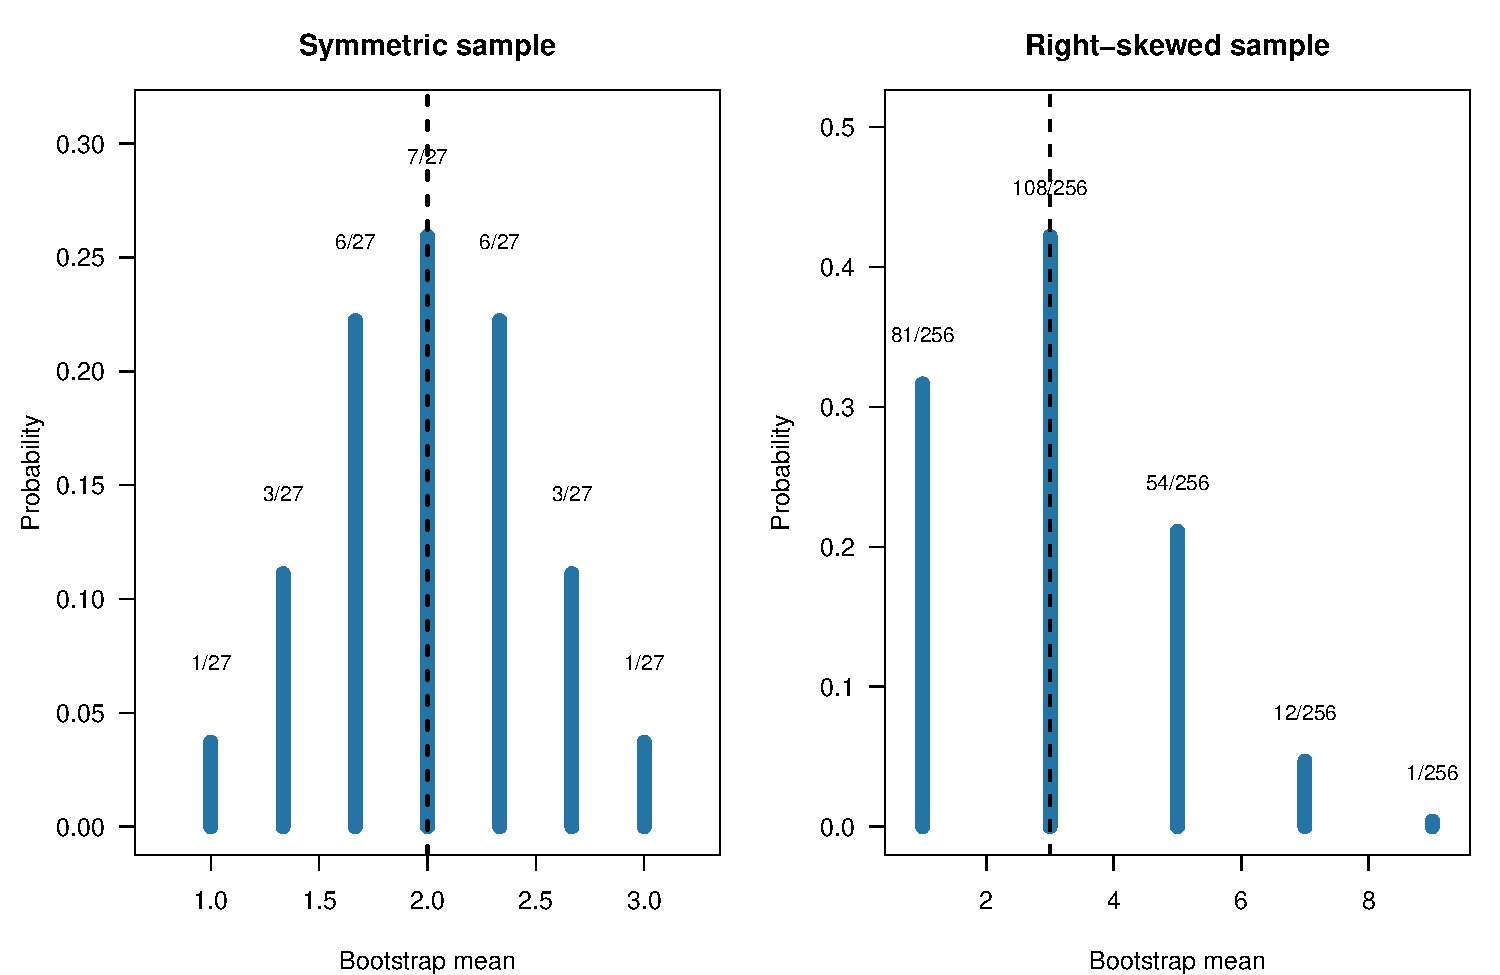
\includegraphics[width=0.95\textwidth]{../../assets/simulate-results/example-bootstrap-distributions.pdf}
\caption{Phân phối Bootstrap chính xác của trung bình trong mẫu đối xứng và mẫu lệch phải; đường đứt biểu thị trung bình mẫu.}
\label{fig:example-bootstrap-distributions}
\end{figure}

Bảng~\ref{fig:example-bootstrap-distributions} cho thấy ví dụ thứ nhất có
phân phối đối xứng quanh $2$, còn ví dụ thứ hai có khối xác suất kéo dài
về phía phải. Bảng~\ref{tab:example-confidence-intervals} cho thấy ba
phương pháp cho các cận khác nhau ở ví dụ lệch; lựa chọn khoảng cần dựa
trên giả định và hiệu năng thực nghiệm, không chỉ dựa vào hình dạng của
một phân phối Bootstrap.

\newpage
\section{NGHIÊN CỨU MÔ PHỎNG MONTE CARLO BẰNG R}

\subsection{Thiết kế mô phỏng}

Mô phỏng đánh giá coverage và độ dài trung bình của Normal, Basic và
Percentile CI với mức tin cậy danh nghĩa $95\%$. Mỗi trong bốn kịch bản
được lặp $K=10{,}000$ lần; mỗi lần lặp tạo $B=1{,}999$ mẫu Bootstrap~\cite{buithuytrang2026,davison1997,justus2024}.
Các kịch bản gồm tổng thể chuẩn $N(0,1)$ và mũ $\operatorname{Exp}(1)$,
đều ở hai cỡ mẫu $n=12$ và $n=40$. Seed được cố định ở $20260925$ để có
thể tái lập kết quả.

Coverage là tỷ lệ các khoảng chứa tham số thật; độ dài trung bình là trung
bình của $U_k-L_k$ qua các lần lặp. Sai số chuẩn Monte Carlo của coverage
được ước lượng bởi
\[
\widehat{MCSE}=\sqrt{\widehat{CP}(1-\widehat{CP})/K}.
\]
Trong ví dụ liệt kê chính xác ở Phần~\ref{sec:examples}, phân vị dùng
quy ước type~1; mô phỏng dùng phân vị nội suy type~7 của R. Tệp
\texttt{run-info.txt} trong thư mục kết quả ghi lại các thiết lập này.

Đoạn mã sau thể hiện phần tính các cận từ một mẫu Bootstrap. Vòng lặp đầy
đủ qua bốn kịch bản, tổng hợp chỉ số và xuất kết quả được triển khai trong
mã mô phỏng R.

\begin{lstlisting}[style=Rstyle, caption={Tính các khoảng tin cậy}]
x <- c(1, 2, 3, 4, 5)
n <- length(x)
B <- 1000
alpha <- 0.05

theta_hat <- mean(x)
boot_means <- colMeans(matrix(sample(x, n * B, replace = TRUE), nrow = n))
se <- sd(boot_means)
q <- quantile(boot_means, c(alpha / 2, 1 - alpha / 2))

ci <- rbind(
  Normal = c(theta_hat - 1.96 * se, theta_hat + 1.96 * se),
  Basic = c(2 * theta_hat - q[2], 2 * theta_hat - q[1]),
  Percentile = c(q[1], q[2])
)
colnames(ci) <- c("Lower", "Upper")
round(ci, 3)
\end{lstlisting}

\subsection{Kết quả mô phỏng}

Bảng~\ref{tab:simulation-results} tổng hợp kết quả từ lần chạy có seed cố
định. Coverage và MCSE được trình bày theo phần trăm; AL giữ nguyên đơn vị
của thống kê trung bình.

\begin{table}[htbp]
\centering
\scriptsize
\renewcommand{\arraystretch}{1.12}
\setlength{\tabcolsep}{4pt}
\caption{Coverage, độ dài khoảng trung bình và MCSE trong mô phỏng ($K=10{,}000$, $B=1{,}999$)}
\label{tab:simulation-results}
\begin{tabular}{llrrr}
\toprule
Phân phối & Phương pháp & Coverage (\%) & AL & MCSE (điểm \%) \\
\midrule
\multirow{3}{*}{$N(0,1),\ n=12$}
& Normal & 91.05 & 1.0585 & 0.29 \\
& Basic & 91.01 & 1.0528 & 0.29 \\
& Percentile & 90.74 & 1.0528 & 0.29 \\
\addlinespace
\multirow{3}{*}{$N(0,1),\ n=40$}
& Normal & 93.91 & 0.6081 & 0.24 \\
& Basic & 93.89 & 0.6065 & 0.24 \\
& Percentile & 93.79 & 0.6065 & 0.24 \\
\addlinespace
\multirow{3}{*}{$\operatorname{Exp}(1),\ n=12$}
& Normal & 87.06 & 1.0153 & 0.34 \\
& Basic & 85.47 & 1.0002 & 0.35 \\
& Percentile & 87.59 & 1.0002 & 0.33 \\
\addlinespace
\multirow{3}{*}{$\operatorname{Exp}(1),\ n=40$}
& Normal & 91.92 & 0.5971 & 0.27 \\
& Basic & 90.99 & 0.5939 & 0.29 \\
& Percentile & 92.21 & 0.5939 & 0.27 \\
\bottomrule
\end{tabular}
\end{table}

\begin{figure}[htbp]
\centering
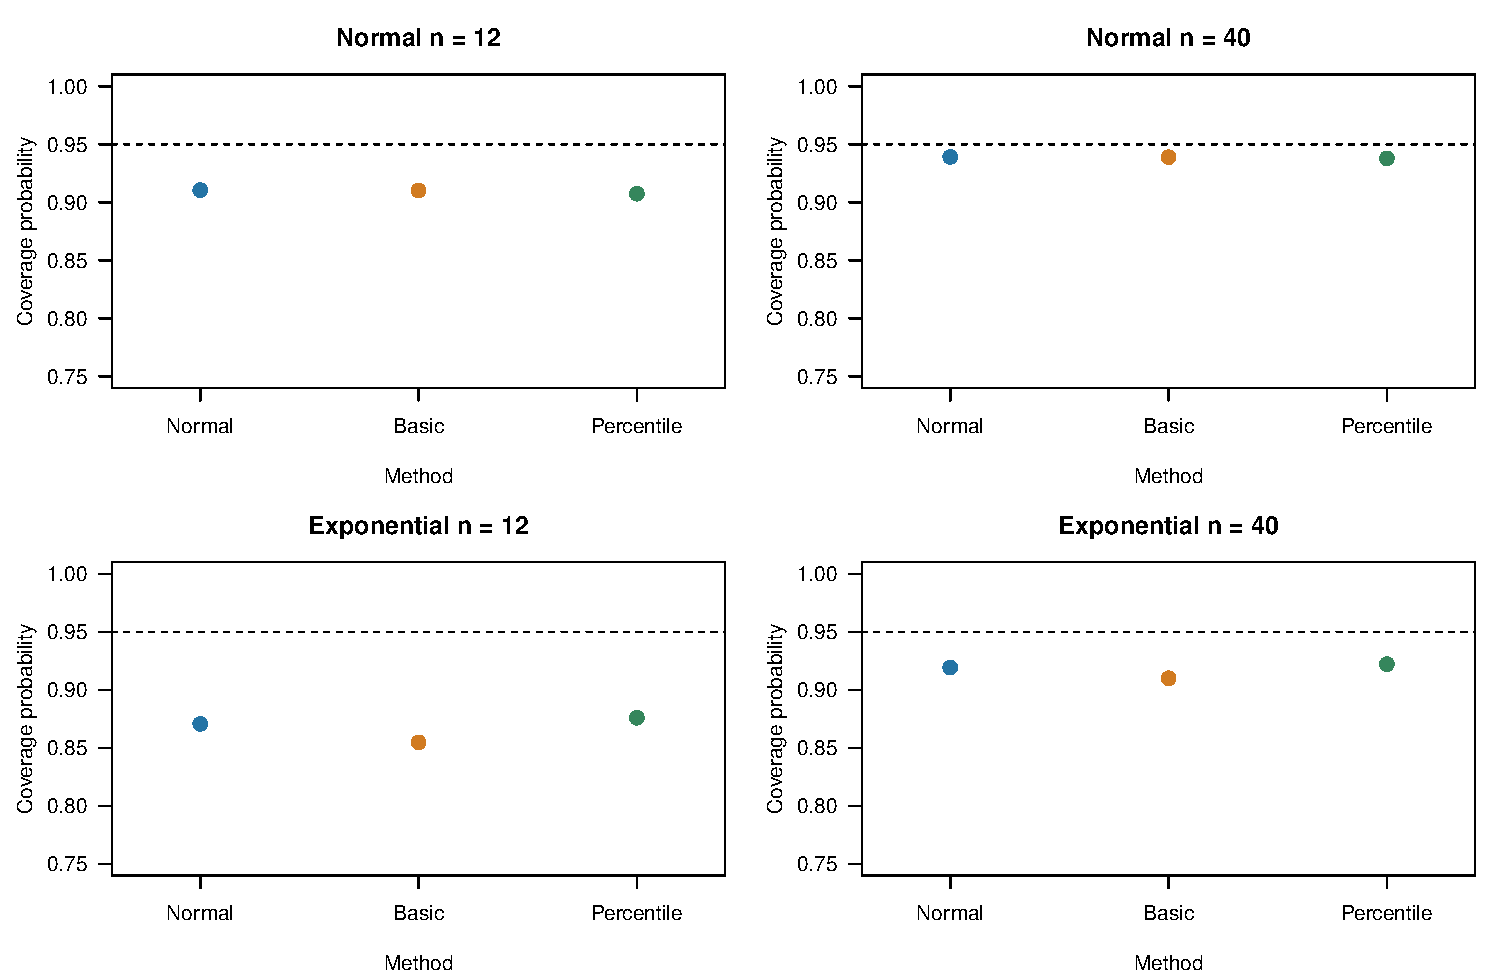
\includegraphics[width=0.95\textwidth]{../../assets/simulate-results/simulation-coverage.pdf}
\caption{Coverage của ba phương pháp trong bốn kịch bản; đường đứt biểu thị mức danh nghĩa $95\%$.}
\label{fig:simulation-coverage}
\end{figure}

\begin{figure}[htbp]
\centering
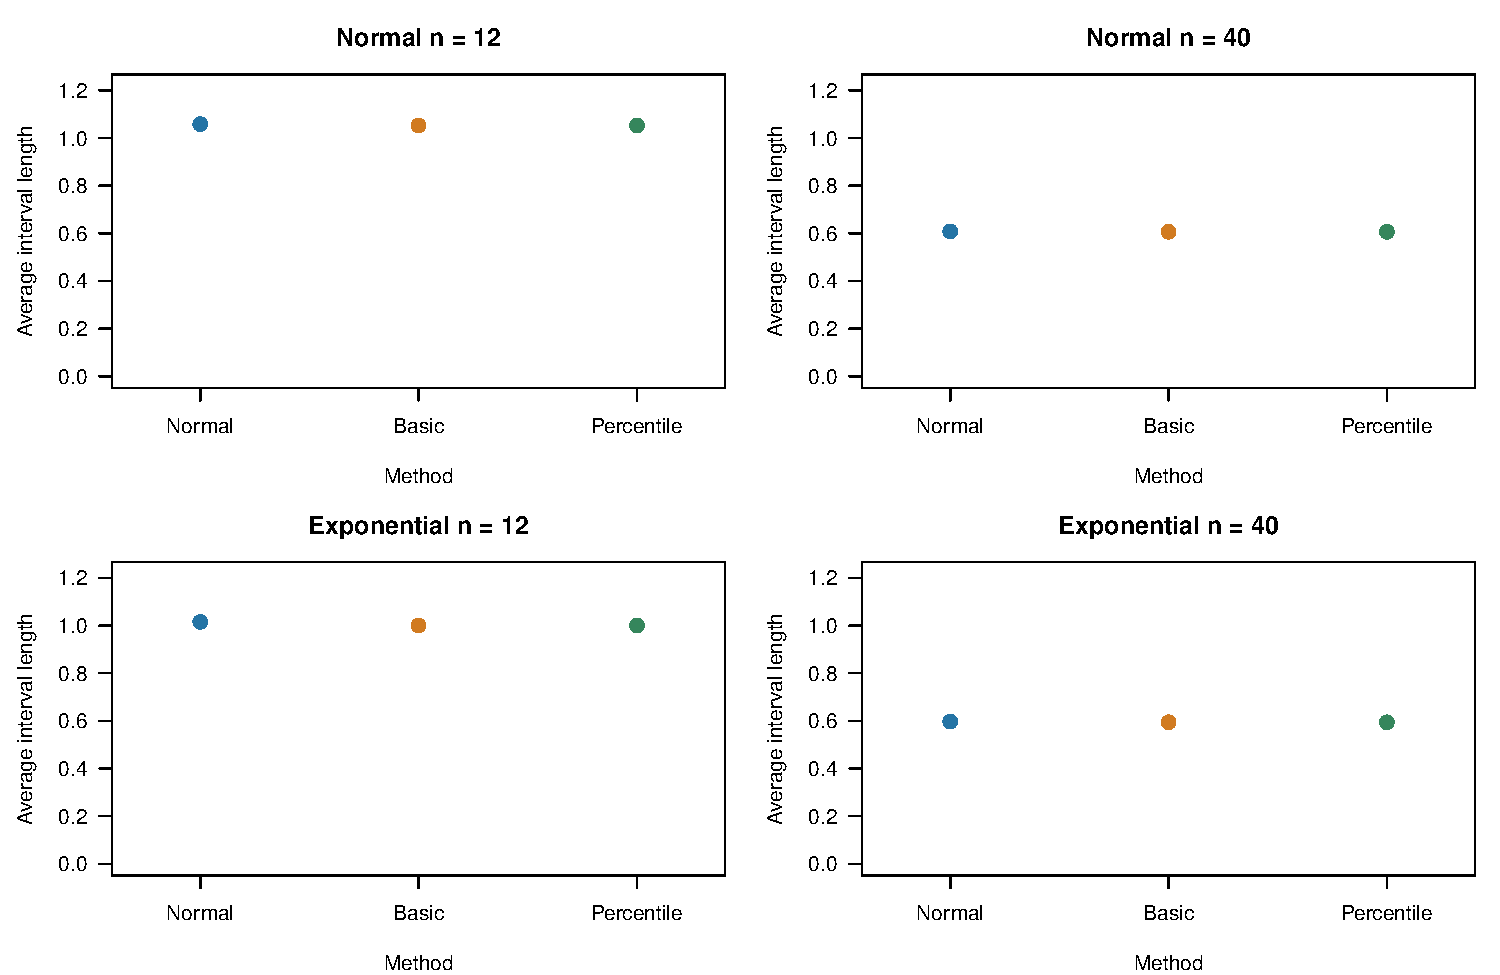
\includegraphics[width=0.95\textwidth]{../../assets/simulate-results/simulation-average-length.pdf}
\caption{Độ dài khoảng trung bình của ba phương pháp trong bốn kịch bản.}
\label{fig:simulation-average-length}
\end{figure}

Trong tổng thể chuẩn, coverage của ba phương pháp khá gần nhau và tăng từ
khoảng $91\%$ ở $n=12$ lên khoảng $94\%$ ở $n=40$. Với tổng thể mũ, ở cả
hai cỡ mẫu, Basic có coverage thấp hơn Normal trong lần mô phỏng này;
Percentile có coverage cao nhất trong ba phương pháp ở cả $n=12$ và $n=40$.
AL của Basic và Percentile trùng nhau trong từng kịch bản do hai khoảng
được phản chiếu từ cùng cặp phân vị. Các kết quả này mô tả đúng bốn kịch
bản đã xét, không khẳng định thứ hạng phương pháp cho mọi phân phối.

\paragraph{Độ bao phủ của Normal Bootstrap với mẫu chuẩn.}
Gọi $S$ là độ lệch chuẩn mẫu với mẫu số $n-1$. Khi giữ $n$ cố định và
$B\to\infty$, sai số chuẩn Bootstrap của trung bình tiến tới
\[
    se_\infty^*=\sqrt{\operatorname{Var}^*(\bar X^*)}
    =\sqrt{\frac{n-1}{n}}\frac{S}{\sqrt n}.
\]
Công thức~\eqref{eq:bootstrap-mean-variance} cho phương sai có điều kiện của $\bar X^*$.
Với $T=(\bar X-\mu)/(S/\sqrt n)\sim t_{n-1}$, độ bao phủ giới hạn là
$\Pr(|T|\le z_{0.975}\sqrt{(n-1)/n})$: $91.27\%$ ở $n=12$ và $93.98\%$
ở $n=40$, so với $91.05\%$ và $93.91\%$ trong Bảng~\ref{tab:simulation-results}.
Mức hụt so với $95\%$ vẫn xuất hiện khi tính chính xác sai số chuẩn Bootstrap.



\newpage
\section{ỨNG DỤNG BOOTSTRAP CI TRONG Y SINH}

\subsection{Bootstrap trong phân tích dữ liệu sống còn}

Dữ liệu sống còn có thể bị kiểm duyệt nếu thời gian theo dõi kết thúc trước khi biến cố xuất hiện hoặc người tham gia rời nghiên cứu. Trong mô hình Cox, Hazard Ratio (HR) là hàm mũ của hệ số hồi quy. Khi Bootstrap được dùng để đánh giá độ bất định của HR, cách lấy mẫu lại cần phù hợp với cấu trúc dữ liệu~\cite[tr. 334--340]{davison1997}.

Với hệ số ước lượng $\widehat{\beta}$, $\widehat{HR}=\exp(\widehat{\beta})$.
Khoảng Wald được tính trên thang log-HR rồi chuyển về thang HR:
\[
\left[
\exp(\widehat{\beta}-z_{1-\alpha/2}SE(\widehat{\beta})),
\exp(\widehat{\beta}+z_{1-\alpha/2}SE(\widehat{\beta}))
\right].
\]
Do phép biến đổi hàm mũ, hai cận của khoảng Wald Cox trên thang HR đều dương.
Normal Bootstrap CI tính trực tiếp trên thang HR là một cách xây dựng khác.

\subsection{Ví dụ giả định: ước lượng Hazard Ratio}

\textit{Ví dụ dưới đây dùng số liệu giả định để minh họa phép tính, không mô tả
một nghiên cứu hay thử nghiệm lâm sàng cụ thể.}

Quy trình minh họa gồm các bước sau:
\begin{enumerate}
	\item \textbf{Ước lượng Hazard Ratio:} Đặt $HR=h_{\text{điều trị}}/h_{\text{đối chứng}}$ và giả sử ước lượng trên mẫu gốc là $\widehat{HR}_n=1.85$. Nếu biến cố là tử vong, giá trị này biểu thị hazard tử vong tức thời ở nhóm điều trị cao hơn nhóm đối chứng theo mô hình Cox; cách diễn giải phụ thuộc vào quy ước mã hóa nhóm và biến cố.
	\item \textbf{Bootstrap phân tầng ($B=2000$):} Rút $2000$ mẫu Bootstrap phân tầng (stratified bootstrap), lấy mẫu riêng trong từng nhóm để giữ nguyên cỡ nhóm~\cite[tr. 86--91]{davison1997}. Với mỗi mẫu $b$, tính lại $\widehat{\text{HR}}^{*(b)}$.
	\item \textbf{Phân phối Bootstrap giả định:} Giả sử phân phối các bản sao $\widehat{\text{HR}}^*$ lệch phải và có các đặc trưng sau:
	\begin{itemize}
		\item Sai số chuẩn Bootstrap: $\widehat{se}^* = 0.42$.
		\item Phân vị dưới $2.5\%$: $q_{0.025}^* = 1.15$.
		\item Phân vị trên $97.5\%$: $q_{0.975}^* = 2.82$.
	\end{itemize}
	\item \textbf{Xây dựng và So sánh các Khoảng tin cậy $95\%$:}
	\begin{itemize}
		\item \textbf{Normal Bootstrap CI:}
		\begin{equation}
			CI_{\text{Normal}} = [1.85 - 1.96 \times 0.42, \quad 1.85 + 1.96 \times 0.42] = [1.027, \quad 2.673]
		\end{equation}
		\item \textbf{Basic Bootstrap CI (Quantile Flipping):}
		\begin{equation}
			CI_{\text{Basic}} = [2(1.85) - 2.82, \quad 2(1.85) - 1.15] = [0.880, \quad 2.550]
		\end{equation}
	\end{itemize}
\end{enumerate}

\textbf{Diễn giải:}
\begin{itemize}
	\item Hai khoảng thu được là
	$CI_{\text{Normal}}=[1.027,2.673]$ và
	$CI_{\text{Basic}}=[0.880,2.550]$. Trong ví dụ này, khoảng Normal
	không chứa $1$, còn khoảng Basic có chứa $1$.

	\item Hai khoảng đưa ra kết luận khác nhau về việc giá trị tham chiếu $1$
	có nằm trong khoảng hay không. Do số liệu được giả định, ví dụ này chỉ
	minh họa phép tính, không đánh giá độ chính xác hay xác suất bao phủ của
	hai phương pháp.

	\item Với dữ liệu sống còn thực tế, đơn vị lấy mẫu Bootstrap là bệnh nhân:
	mỗi lần lấy mẫu cần giữ đi cùng thời gian theo dõi, trạng thái biến cố
	và nhóm điều trị của bệnh nhân. Sau đó khớp lại mô hình Cox trên từng
	mẫu Bootstrap; cần báo cáo số mẫu không hội tụ nếu có.
\end{itemize}
\subsection{Bài báo khoa học: khoảng Bootstrap cho relative validity}

Deng và cộng sự (2013) dùng Bootstrap để đánh giá ý nghĩa thống kê của
relative validity (RV) và khảo sát các yếu tố ảnh hưởng đến kết luận.
Phân tích dựa trên câu trả lời của 453 bệnh nhân bệnh thận mạn đối với 16
thang đo đặc hiệu và tổng quát; RV cho biết mỗi thang đo phân biệt các
nhóm lâm sàng tốt đến mức nào so với thang đo tham chiếu~\cite[tr. 2--4]{deng2013}.

Đại lượng chính là relative validity (RV), được tính bằng tỷ số giữa
thống kê $F$ của công cụ so sánh và thống kê $F$ của công cụ tham chiếu:
\[
RV =
\frac{F_{\text{công cụ so sánh}}}
{F_{\text{công cụ tham chiếu}}}.
\]
Công cụ QDIS-CKD CAT-5 được chọn làm tham chiếu, có $F=57.43$ và
$RV=1$. Giá trị $RV<1$ biểu thị công cụ so sánh phân biệt các nhóm kém
hơn công cụ tham chiếu theo tiêu chí này.

Bài báo sử dụng khoảng tin cậy Bootstrap $95\%$ cho RV. Chú thích bảng
kết quả xác định đây là khoảng BCa (Bias-Corrected and Accelerated),
không phải Normal CI hay Basic CI. Bảng dưới đây trích một số kết quả
đại diện từ nghiên cứu~\cite[Bảng 1, tr.~3]{deng2013}.

\begin{table}[htbp]
	\centering
	\small
	\renewcommand{\arraystretch}{1.2}
	\setlength{\tabcolsep}{6pt}
	\caption{Một số kết quả RV và khoảng tin cậy BCa trong nghiên cứu của Deng và cộng sự}
	\label{tab:deng-bca}
	\begin{tabular}{l c c c >{\raggedright\arraybackslash}p{6.8cm}}
		\toprule
		\textbf{Công cụ so sánh} &
		\textbf{$F$} &
		\textbf{RV} &
		\textbf{BCa 95\% CI} &
		\textbf{Diễn giải so với tham chiếu} \\
		\midrule
		QDIS-CKD Static-6 & 50.15 & 0.87 & [0.72; 1.03] &
		Khoảng chứa 1; chưa cho thấy khác biệt rõ ở mức 5\%. \\

		QDIS-CKD Static-34 & 48.01 & 0.84 & [0.71; 0.97] &
		Khoảng nằm dưới 1; RV thấp hơn tham chiếu theo khoảng BCa. \\

		KDQOL Burden & 44.46 & 0.77 & [0.53; 1.09] &
		Khoảng chứa 1; chưa cho thấy khác biệt rõ ở mức 5\%. \\

		KDQOL Symptoms & 15.11 & 0.26 & [0.13; 0.44] &
		Khoảng nằm dưới 1; RV thấp hơn tham chiếu theo khoảng BCa. \\
		\bottomrule
	\end{tabular}
\end{table}

Bảng \ref{tab:deng-bca} cho thấy chỉ nhìn vào RV điểm là chưa đủ để
kết luận hai công cụ khác nhau. Chẳng hạn, RV của KDQOL Burden bằng
$0.77$, nhưng khoảng BCa $[0.53;1.09]$ vẫn chứa giá trị tham chiếu $1$.
Ngược lại, khoảng của QDIS-CKD Static-34 là $[0.71;0.97]$, không chứa
$1$. Vì vậy, theo cách diễn giải khoảng tin cậy trong nghiên cứu,
Static-34 có RV thấp hơn có ý nghĩa thống kê so với công cụ tham chiếu,
còn kết quả của KDQOL Burden chưa đủ để đưa ra kết luận tương tự~\cite{deng2013}.

Nghiên cứu còn thực hiện mô phỏng để khảo sát ảnh hưởng của cỡ mẫu,
thống kê $F$ của công cụ tham chiếu, tương quan giữa hai công cụ và số
lần lấy mẫu Bootstrap. Một kết quả đáng chú ý là khi $F$ của công cụ
tham chiếu khoảng $57$ và tương quan giữa hai công cụ bằng $0.7$, công
suất đạt khoảng $80\%$ để phát hiện RV xấp xỉ $0.6$. Tác giả cũng nhận
xét rằng tăng số lần lặp Bootstrap vượt quá $500$ đem lại ít thay đổi
trong các kịch bản mô phỏng của bài báo~\cite{deng2013}.

Ví dụ này minh họa BCa được dùng để lượng hóa độ bất định của một tỷ số
thống kê phức tạp. Tuy nhiên, bài báo không phải là phép so sánh trực
tiếp BCa với Normal CI và Basic CI. Do đó, kết quả này bổ sung ví dụ ứng
dụng thực tế cho báo cáo, còn việc so sánh Normal CI và Basic CI vẫn
được thực hiện riêng trong phần mô phỏng của nhóm.

\begin{lstlisting}[style=Rstyle, caption={Vẽ lại các khoảng BCa được công bố trong bài báo}, label={lst:deng-bca}]
measure <- c("KDQOL Symptoms", "KDQOL Burden", "QDIS Static-34", "QDIS Static-6")
rv <- c(0.26, 0.77, 0.84, 0.87)
lower <- c(0.13, 0.53, 0.71, 0.72)
upper <- c(0.44, 1.09, 0.97, 1.03)
y <- 1:4

par(mar = c(4, 9, 2, 1))
plot(rv, y, xlim = c(0, 1.3), ylim = c(0.5, 4.5), yaxt = "n", pch = 19,
     xlab = "Relative validity (RV) & BCa 95% CI", ylab = "")
axis(2, at = y, labels = measure, las = 1)
segments(lower, y, upper, y, lwd = 2)
abline(v = 1, lty = 2, col = "red")
\end{lstlisting}

\subsection{Mã R minh họa Bootstrap cho Hazard Ratio}

Mã ở Listing~\ref{lst:deng-bca} chỉ vẽ lại các ước lượng RV và cận BCa đã công bố; mã không tái lập phân tích từ dữ liệu gốc. Mã tiếp theo tạo dữ liệu giả định, khớp mô hình Cox và lấy mẫu lại phân tầng theo nhóm để minh họa việc tính Normal CI và Basic CI; đây không phải phân tích dữ liệu của nghiên cứu Deng và cộng sự:

\begin{lstlisting}[style=Rstyle, caption={Bootstrap HR}]
library(survival)
set.seed(2026)
n <- 40
group <- rep(c(0, 1), each = 20)
time <- rexp(n, rate = 0.1 * exp(-0.6 * group))
status <- rbinom(n, size = 1, prob = 0.85)
data_med <- data.frame(time, status, group)

fit <- coxph(Surv(time, status) ~ group, data = data_med)
hr_hat <- exp(coef(fit))

B <- 500
boot_hr <- numeric(B)
g0 <- which(group == 0)
g1 <- which(group == 1)

for (b in 1:B) {
  idx <- c(sample(g0, replace = TRUE), sample(g1, replace = TRUE))
  fit_b <- coxph(Surv(time[idx], status[idx]) ~ group[idx])
  boot_hr[b] <- exp(coef(fit_b))
}

se <- sd(boot_hr)
q <- quantile(boot_hr, c(0.025, 0.975))

ci <- rbind(
  Normal = c(hr_hat - 1.96 * se, hr_hat + 1.96 * se),
  Basic = c(2 * hr_hat - q[2], 2 * hr_hat - q[1]),
  Percentile = c(q[1], q[2])
)
colnames(ci) <- c("Lower", "Upper")
round(ci, 3)
\end{lstlisting}

% ==================== PHẦN 8 ====================

\newpage
\section{NỘI DUNG MỞ RỘNG: PERCENTILE CI VÀ TÍNH BẤT BIẾN}

\subsection{Khoảng tin cậy Bootstrap phân vị (Percentile CI)}

Bên cạnh Normal CI và Basic CI, Percentile CI lấy trực tiếp các phân vị của phân phối Bootstrap làm hai cận khoảng~\cite{rizzo2019,efron1993,quyen2025}.

\subsubsection{Cơ sở và công thức}
Percentile CI dùng trực tiếp hai phân vị của các bản sao. Khi sai số
Bootstrap gần đối xứng quanh $0$, hai phân vị thỏa xấp xỉ
$q_L^*+q_U^*\approx2\hat\theta_n$, nên các cận gần với Basic CI.
Lập luận có thể áp dụng trên một thang biến đổi đơn điệu thích hợp~\cite[tr.~160--163]{efron1993}.

\begin{equation}
	CI_{\text{Percentile}} = \left[ q_{\alpha/2}^*, \quad q_{1-\alpha/2}^* \right]
\end{equation}
trong đó $q_{\alpha/2}^*$ và $q_{1-\alpha/2}^*$ tương ứng là phân vị thực nghiệm mức $\alpha/2$ và $1-\alpha/2$ của các bản sao Bootstrap~\cite{buithuytrang2026,rizzo2019}.
\subsection{Khoảng tin cậy Bootstrap BCa}

Khoảng tin cậy Bootstrap BCa (Bias-Corrected and Accelerated) điều chỉnh
các phân vị Bootstrap để phản ánh độ chệch và độ bất đối xứng của phân phối
ước lượng~\cite{efron1993,davison1997}.

Gọi $\hat{\theta}_n$ là ước lượng từ mẫu gốc và
$\hat{\theta}^{*(1)},\ldots,\hat{\theta}^{*(B)}$ là các bản sao Bootstrap.
Hệ số hiệu chỉnh độ chệch được ước lượng bởi:
\begin{equation}
	\widehat{z}_0
	=
	\Phi^{-1}\left(
	\frac{1}{B}\sum_{b=1}^{B}
	\mathbf{1}\left\{
	\hat{\theta}^{*(b)} < \hat{\theta}_n
	\right\}
	\right),
\end{equation}
trong đó $\Phi^{-1}$ là hàm phân vị của phân phối Chuẩn tắc.

Tiếp theo, gọi $\hat{\theta}_{(i)}$ là giá trị thống kê tính khi bỏ quan sát
thứ $i$ khỏi mẫu, và
$\bar{\theta}_{(.)}=n^{-1}\sum_{i=1}^{n}\hat{\theta}_{(i)}$. Hệ số gia tốc
được ước lượng bằng:
\begin{equation}
	\widehat{a}
	=
	\frac{
		\displaystyle\sum_{i=1}^{n}
		\left(\bar{\theta}_{(.)}-\hat{\theta}_{(i)}\right)^3
	}{
		\displaystyle
		6\left[
		\sum_{i=1}^{n}
		\left(\bar{\theta}_{(.)}-\hat{\theta}_{(i)}\right)^2
		\right]^{3/2}
	}.
\end{equation}

Với mức ý nghĩa $\alpha$, hai mức phân vị điều chỉnh được xác định bởi:
\begin{equation}
	p_L
	=
	\Phi\left[
	\widehat{z}_0+
	\frac{\widehat{z}_0+z_{\alpha/2}}
	{1-\widehat{a}(\widehat{z}_0+z_{\alpha/2})}
	\right],
\end{equation}
\begin{equation}
	p_U
	=
	\Phi\left[
	\widehat{z}_0+
	\frac{\widehat{z}_0+z_{1-\alpha/2}}
	{1-\widehat{a}(\widehat{z}_0+z_{1-\alpha/2})}
	\right],
\end{equation}
trong đó $z_p=\Phi^{-1}(p)$. Hai mức $p_L$ và $p_U$ nói chung không có tổng bằng $1$. Khoảng tin cậy BCa được tính bằng:
\begin{equation}
	CI_{\mathrm{BCa}}
	=
	\left[
	q_{p_L}^{*},
	q_{p_U}^{*}
	\right].
\end{equation}

Các công thức trên yêu cầu $\widehat z_0$ hữu hạn, mẫu Jackknife không suy biến và các mẫu số của phép hiệu chỉnh khác $0$. Nếu các điều kiện này không thỏa mãn, cần kiểm tra tính khả dụng của BCa trước khi báo cáo khoảng.

Percentile CI lấy trực tiếp hai phân vị Bootstrap thông thường, còn BCa
điều chỉnh các mức phân vị để xét đến độ chệch và độ bất đối xứng.
BCa có thể cải thiện độ chính xác trong những điều kiện thích hợp, nhưng
không bảo đảm tốt hơn trong mọi trường hợp; kết quả còn phụ thuộc vào dữ
liệu, thống kê đang xét và số lần lấy mẫu Bootstrap~\cite{efron1993,davison1997}.
\subsection{So sánh Normal CI, Basic CI và Percentile CI}

Bảng \ref{tab:trio_comparison} so sánh ba phương pháp khoảng tin cậy Bootstrap~\cite{buithuytrang2026,rizzo2019,efron1993,davison1997,justus2024}. Đặt $q_L^*=q_{\alpha/2}^*$ và $q_U^*=q_{1-\alpha/2}^*$.

\begin{table}[htbp]
	\centering
	\small
	\renewcommand{\arraystretch}{1.4}
	\setlength{\tabcolsep}{4pt}
	\caption{So sánh Normal CI, Basic CI và Percentile CI}
	\label{tab:trio_comparison}
	\begin{tabular}{>{\raggedright\arraybackslash}p{2.5cm}>{\raggedright\arraybackslash}p{4.2cm}>{\raggedright\arraybackslash}p{4.2cm}>{\raggedright\arraybackslash}p{4.2cm}}
		\toprule
		\textbf{Tiêu chí} & \textbf{Normal CI} & \textbf{Basic CI} & \textbf{Percentile CI} \\
		\midrule
		\textbf{Công thức} & $\hat{\theta}_n \pm z_{1-\alpha/2}\widehat{se}^*$  & $[2\hat{\theta}_n-q_U^*,\;2\hat{\theta}_n-q_L^*]$  & $[q_L^*,q_U^*]$  \\
		\textbf{Cơ sở} & Dựa trên xấp xỉ chuẩn của ước lượng. & Dựa trên xấp xỉ phân phối sai số Bootstrap. & Dùng trực tiếp các phân vị Bootstrap. \\
		\textbf{Phân phối lệch phải} & Khoảng đối xứng quanh $\hat{\theta}_n$. & Quantile Flipping có thể tạo khoảng bất đối xứng. & Hai cận theo hướng phân phối Bootstrap. \\
		\textbf{Bất biến qua $g(\theta)$} & Nói chung không bất biến. & Nói chung không bất biến. & Bất biến qua biến đổi đơn điệu, nếu quy tắc phân vị tương thích. \\
		\textbf{Độ chính xác tiệm cận} & Bậc nhất, tùy điều kiện. & Bậc nhất, tùy điều kiện. & Bậc nhất, tùy điều kiện. \\
		\bottomrule
	\end{tabular}
\end{table}

\subsection{Tính bất biến dưới phép biến đổi tham số $g(\theta)$}

\begin{definition}[\textbf{Tính Bất biến của Khoảng Tin cậy}]
	Một phương pháp xây dựng khoảng tin cậy cho tham số $\theta$ được gọi là \textbf{bất biến (invariant)} dưới phép biến đổi đơn điệu $g(\cdot)$ nếu khoảng tin cậy cho tham số mới $\eta = g(\theta)$ đúng bằng việc áp dụng ánh xạ $g(\cdot)$ lên các cận của khoảng tin cậy cho $\theta$~\cite[Section 13.3, tr. 162--163]{efron1993}:
	\begin{equation}
		CI_{g(\theta)} =
    \begin{cases}
      [g(L_{\theta}),g(U_{\theta})], & g\ \text{đồng biến},\\
      [g(U_{\theta}),g(L_{\theta})], & g\ \text{nghịch biến}.
    \end{cases}
	\end{equation}
	\end{definition}

		\subsubsection{Tính bất biến của Percentile CI}
		Giả sử $g(\cdot)$ là một hàm số đồng biến nghiêm ngặt (strictly monotonic increasing function), chẳng hạn như phép biến đổi Logarithm $g(x) = \ln(x)$ hoặc phép biến đổi Lũy thừa $g(x) = x^2$ với $x > 0$.
		Trong chứng minh này, dùng phân vị thực nghiệm type~1 (nghịch đảo tổng quát của ECDF), không nội suy giữa hai giá trị. Với nội suy tuyến tính type~7, phép biến đổi phi tuyến nói chung không giao hoán với nội suy. Vì $g(\cdot)$ đồng biến, thứ tự các phần tử trong tập hợp bản sao Bootstrap được giữ nguyên hoàn toàn~\cite[tr. 162--163]{efron1993}:
		\begin{equation}
			\hat{\theta}^{*(1)} \le \hat{\theta}^{*(2)} \le \dots \le \hat{\theta}^{*(B)} \iff g(\hat{\theta}^{*(1)}) \le g(\hat{\theta}^{*(2)}) \le \dots \le g(\hat{\theta}^{*(B)})
		\end{equation}
		Do đó, phân vị thực nghiệm mức $p$ của tham số mới $g(\hat{\theta}^*)$ chính bằng giá trị $g(\cdot)$ áp dụng lên phân vị thực nghiệm mức $p$ của $\hat{\theta}^*$~\cite[tr. 162--163]{efron1993}:
		\begin{equation}
			q_p^*\left(g(\hat{\theta}^*)\right) = g\left(q_p^*(\hat{\theta}^*)\right)
		\end{equation}

		Từ đó, khoảng tin cậy Percentile CI cho tham số $g(\theta)$ là~\cite{rizzo2019,efron1993}:
		\begin{equation}
			CI_{\text{Percentile}}(g(\theta)) = \left[ q_{\alpha/2}^*(g(\hat{\theta}^*)), \quad q_{1-\alpha/2}^*(g(\hat{\theta}^*)) \right] = \left[ g(q_{\alpha/2}^*), \quad g(q_{1-\alpha/2}^*) \right] \quad (\text{đpcm})
		\end{equation}

		\subsubsection{Normal CI và Basic CI dưới phép biến đổi phi tuyến}
		Với phép biến đổi phi tuyến, Normal CI và Basic CI nói chung không bất biến~\cite{rizzo2019,efron1993,davison1997}:
		\begin{itemize}
			\item \textbf{Normal CI:} Sai số chuẩn và phép biến đổi phi tuyến nói chung không giao hoán; khoảng tính trực tiếp trên thang mới có thể khác với khoảng cũ sau biến đổi~\cite[tr. 163]{efron1993}.
			\item \textbf{Basic CI:} Phép phản chiếu phân vị quanh ước lượng điểm nói chung không giao hoán với phép biến đổi phi tuyến~\cite[tr. 203]{davison1997}.
		\end{itemize}

		\subsubsection{Kiểm chứng bằng phép biến đổi log}

Dùng cùng các bản sao Bootstrap của mẫu dương $(2,3,4,5,9)$ để so sánh
khoảng tính trên thang $\theta$ rồi lấy log với khoảng tính trực tiếp
trên thang $\eta=\log(\theta)$. Phân vị dùng type~1 trong kiểm chứng này,
để phép biến đổi đơn điệu tăng bảo toàn thứ tự và phân vị thực nghiệm. Đoạn mã là trích đoạn của \texttt{r/Nhom\_D\_TKTT.R}; để tái lập các số ở Bảng~\ref{tab:invariance-log}, chạy toàn bộ tệp với seed và chuỗi mô phỏng đã nêu ở Phần 6.

\begin{lstlisting}[style=Rstyle, caption={Bất biến dưới log}]
x <- c(2, 3, 4, 5, 9)
n <- length(x)
B <- 1000

boot_theta <- colMeans(matrix(sample(x, n * B, replace = TRUE), nrow = n))
boot_eta <- log(boot_theta)

theta_hat <- mean(x)
eta_hat <- log(theta_hat)

q_theta <- quantile(boot_theta, c(0.025, 0.975), type = 1)
q_eta <- quantile(boot_eta, c(0.025, 0.975), type = 1)

diff_percentile <- max(abs(log(q_theta) - q_eta))

ci_basic_theta <- c(2 * theta_hat - q_theta[2], 2 * theta_hat - q_theta[1])
ci_basic_eta <- c(2 * eta_hat - q_eta[2], 2 * eta_hat - q_eta[1])
diff_basic <- max(abs(log(ci_basic_theta) - ci_basic_eta))

result <- c(Percentile_Diff = diff_percentile, Basic_Diff = diff_basic)
round(result, 6)
\end{lstlisting}

\begin{table}[htbp]
\centering
\small
\caption{Sai khác lớn nhất giữa hai cách tính khoảng trên thang log}
\label{tab:invariance-log}
\begin{tabular}{lrr}
\toprule
Phương pháp & Sai khác lớn nhất & Khớp trong sai số $10^{-12}$ \\
\midrule
Normal & 0.1566453 & Không \\
Basic & 0.3177451 & Không \\
Percentile & 0 & Có \\
\bottomrule
\end{tabular}
\end{table}

\begin{figure}[htbp]
\centering
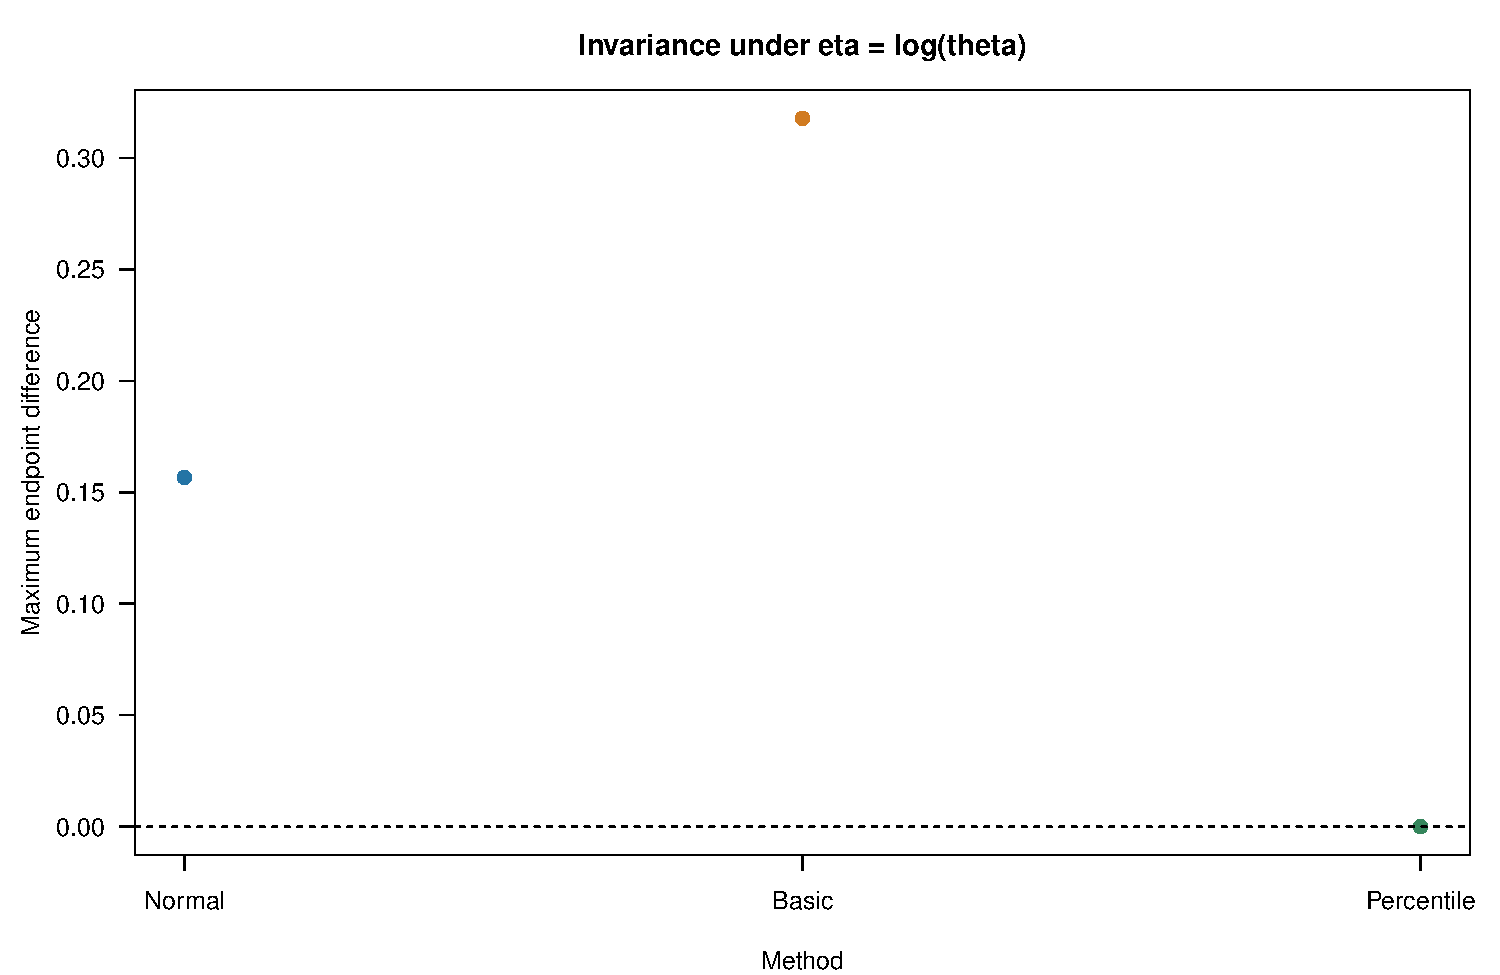
\includegraphics[width=0.78\textwidth]{../../assets/simulate-results/invariance-log-comparison.pdf}
\caption{Sai khác giữa hai cách tính khoảng sau phép biến đổi $\eta=\log(\theta)$.}
\label{fig:invariance-log}
\end{figure}

Trên mẫu đã chọn, hai cách tính Percentile trùng nhau đến sai số máy.
Normal và Basic cho cận khác nhau. Với $g$ giảm, phân vị type~1 ở mức $p$
trên thang mới lấy phần tử gốc có hạng $B+1-\lceil Bp\rceil$. Khoảng tính
lại chỉ khớp với phép đảo hai cận khi hạng này tương thích với hạng
$\lceil B(1-p)\rceil$.

% ==================== PHẦN 9 ====================

\newpage
	\section{KẾT LUẬN VÀ KHUYẾN NGHỊ THỰC HÀNH}

	\subsection{Kết quả chính}

	Báo cáo trình bày cơ sở Bootstrap, ba cách xây dựng khoảng tin cậy, hai ví dụ liệt kê chính xác và mô phỏng Monte Carlo với $K=10{,}000$ lần lặp. Các kết luận sau được giới hạn trong phạm vi đó~\cite{buithuytrang2026,efron1993,davison1997}:

	\begin{enumerate}
		\item Phân phối thực nghiệm xác định phân phối Bootstrap có điều kiện; số lần lấy mẫu hữu hạn tạo thêm sai số Monte Carlo. Độ chính xác của xấp xỉ còn phụ thuộc vào mẫu và thống kê đang xét~\cite{efron1993}.
		\item Basic CI phản chiếu các phân vị Bootstrap quanh $\hat{\theta}_n$ và có thể tạo khoảng bất đối xứng. Trong các kịch bản mô phỏng của báo cáo, coverage của Basic thấp hơn Normal ở cả hai mẫu từ phân phối mũ.
		\item \textbf{Tính bất biến của Percentile CI:} Với phép biến đổi đơn điệu tăng và quy ước phân vị tương thích, hai cận Percentile biến đổi theo cùng hàm $g$. Ví dụ log minh họa tính chất này trên mẫu đã chọn; với phép biến đổi giảm, cần đảo thứ tự hai cận.
	\end{enumerate}

	\subsection{Sơ đồ lựa chọn phương pháp}

	Sơ đồ dưới đây tóm tắt các yếu tố liên quan đến việc chọn khoảng tin cậy. Lựa chọn cần phù hợp với mô hình, dữ liệu và mục tiêu suy luận~\cite{efron1993,davison1997}. Với dữ liệu phụ thuộc hoặc ngoại lai, cần kiểm tra mô hình và cơ chế lấy mẫu lại trước khi sử dụng sơ đồ.

	\begin{figure}[H]
		\centering
		\begin{adjustbox}{max width=\textwidth}
			\begin{tikzpicture}[
				node distance=1.5cm and 1.8cm,
				font=\small,
				start/.style={
					rectangle, rounded corners=3pt, draw=blue!60!black,
					fill=blue!8, text width=5.2cm, minimum height=1cm,
					align=center, very thick
				},
				decision/.style={
					diamond, aspect=2.1, draw=orange!75!black,
					fill=orange!12, text width=3.3cm, align=center,
					inner sep=2pt, thick
				},
				outcome/.style={
					rectangle, rounded corners=3pt, draw=green!50!black,
					fill=green!8, text width=3.8cm, minimum height=1cm,
					align=center, thick
				},
				arrow/.style={draw, -stealth, thick},
				label/.style={fill=white, inner sep=2pt, font=\footnotesize}
				]

				\node[start] (start) {Chọn phương pháp xây dựng khoảng tin cậy};
				\node[decision, below=of start] (skew)
				{Xấp xỉ chuẩn của thống kê có hợp lý?};

				\node[outcome, below left=1.8cm and 2.0cm of skew] (normal)
				{\textbf{Cân nhắc Normal CI}\\Kiểm tra độ chệch và coverage};

				\node[decision, below right=1.8cm and 2.0cm of skew] (inv)
				{Cần tính bất biến dưới phép biến đổi $g(\theta)$?};

				\node[outcome, below left=1.8cm and 1.0cm of inv] (perc)
				{\textbf{Cân nhắc Percentile / BCa}\\Kiểm tra điều kiện và coverage};

				\node[outcome, below right=1.8cm and 1.0cm of inv] (basic)
				{\textbf{So sánh Basic, Percentile, BCa}\\Đánh giá coverage và độ dài};

				\draw[arrow] (start) -- (skew);
				\draw[arrow] (skew) -- node[label, above left] {Có} (normal);
				\draw[arrow] (skew) -- node[label, above right] {Không} (inv);
				\draw[arrow] (inv) -- node[label, above left] {Có} (perc);
				\draw[arrow] (inv) -- node[label, above right] {Không} (basic);

			\end{tikzpicture}
		\end{adjustbox}
		\caption{Sơ đồ cân nhắc phương pháp khoảng tin cậy Bootstrap; không phải quy tắc bảo đảm phương pháp tối ưu.}
		\label{fig:bootstrap-decision}
	\end{figure}

	\newpage
\subsection{Khuyến nghị thực hành}

	Các khuyến nghị dưới đây giới hạn trong các thiết lập của báo cáo~\cite{buithuytrang2026,rizzo2019,efron1993,justus2024}:
	\begin{itemize}
    \item \textbf{Trong các kịch bản đã mô phỏng:} Coverage của cả ba phương pháp thấp hơn mức danh nghĩa $95\%$, nhưng cao hơn ở $n=40$ so với $n=12$. Kết quả chỉ áp dụng cho hai phân phối và hai cỡ mẫu đã xét; chưa đủ căn cứ để kết luận về $n\ge100$.
    \item \textbf{Với dữ liệu lệch và mẫu nhỏ:} Không phương pháp nào luôn dẫn đầu. Trong mô phỏng phân phối mũ ở $n=12$, Percentile có coverage $87.59\%$, Normal $87.06\%$, còn Basic $85.47\%$. Cần cân nhắc coverage, độ dài khoảng, giả định và mục tiêu phân tích; có thể khảo sát BCa như một phương pháp mở rộng.
    \item \textbf{Với tham số được biến đổi $g(\theta)$:} Cần xác định thang tham số phù hợp và miền xác định của phép biến đổi. Percentile có thể giữ quan hệ biến đổi của hai cận khi $g$ đơn điệu tăng và quy tắc phân vị tương thích; với $g$ giảm, cần đảo thứ tự hai cận.
\end{itemize}


	% ==================== TÀI LIỆU THAM KHẢO ====================
	\newpage
	\renewcommand{\refname}{Tài liệu tham khảo}
\begin{thebibliography}{99}
		\small
		\setlength{\itemsep}{1.5pt}
		\setlength{\parskip}{0pt}
		\addcontentsline{toc}{section}{Tài liệu tham khảo}

		\bibitem{buithuytrang2026}
		Bùi Thùy Trang (2026), \textit{Tài liệu bài giảng và Hướng dẫn đề tài báo cáo môn Thống kê Tính toán (C03107) -- Đề tài 8: Khoảng tin cậy Bootstrap chuẩn tắc và Bootstrap cơ bản: Cơ sở lý thuyết, phương pháp xây dựng và đánh giá}, Khoa Toán – Thống kê, Trường Đại học Tôn Đức Thắng, tr.~8.

		\bibitem{rizzo2019}
		Rizzo, M. L. (2019), \textit{Statistical Computing with R}, Second Edition, Chapman \& Hall/CRC Press, Boca Raton, Florida (Chương 8: Bootstrap and Jackknife, tr.~213--244).

		\bibitem{efron1979}
		Efron, B. (1979), ``Bootstrap Methods: Another Look at the Jackknife'', \textit{The Annals of Statistics}, 7(1), pp.~1--26.

		\bibitem{efron1993}
		Efron, B., \& Tibshirani, R. J. (1993), \textit{An Introduction to the Bootstrap}, Chapman \& Hall/CRC, New York (Chương 12--14, tr.~153--188).

		\bibitem{davison1997}
		Davison, A. C., \& Hinkley, D. V. (1997), \textit{Bootstrap Methods and their Application}, Cambridge University Press, Cambridge (Chương 5, tr.~193--211; Chương 9, tr.~334--340).

		\bibitem{justus2024}
		Justus, V. L., Rodrigues, V. B., \& Sousa, A. R. S. (2024), ``Bootstrap confidence intervals: A comparative simulation study'', \textit{arXiv preprint arXiv:2404.12967}, pp.~1--23.

		\bibitem{quyen2025}
		Nguyễn Thị Quyên, Nguyễn Ngân Hà, \& Đoàn Ngọc Diệu Linh (2025), ``Phương pháp Bootstrap và ứng dụng trong bài toán ước lượng'', \textit{Tạp chí Khoa học} (Trường Đại học Hải Phòng), Số 69 (Tháng 01/2025), tr.~31--39.

		\bibitem{deng2013}
		Deng, N., Allison, J. J., Fang, H. J., Ash, A. S., \& Ware, J. E. Jr. (2013), ``Using the bootstrap to establish statistical significance for relative validity comparisons among patient-reported outcome measures'', \textit{Health and Quality of Life Outcomes}, 11, 89. doi:10.1186/1477-7525-11-89.

		\bibitem{bickelfreedman1981}
		Bickel, P. J., \& Freedman, D. A. (1981), ``Some Asymptotic Theory for the Bootstrap'', \textit{The Annals of Statistics}, 9(6), pp.~1196--1217.

		\bibitem{chernick2011}
		Chernick, M. R., \& LaBudde, R. A. (2011), \textit{An Introduction to Bootstrap Methods with Applications to R}, John Wiley \& Sons, Hoboken, New Jersey (Chương 3, tr.~45--74).

		\bibitem{voss2014}
		Voss, J. (2014), \textit{An Introduction to Statistical Computing: A Simulation-based Approach}, John Wiley \& Sons, Chichester, UK (Mục 5.2.1, tr.~115--124).

		\bibitem{robert2010}
		Robert, C. P., \& Casella, G. (2010), \textit{Introducing Monte Carlo Methods with R}, Springer, New York (Chương 3, tr.~63--75).

	\end{thebibliography}

\end{document}
